\section{Rings} 

  We have extensively talked about groups, and now we look at an algebraic structure called a ring that has two operations. As we introduce rings, we will use the integers as the primary structure to demonstrate our theorems, along with the ring of continuous functions and the ring of matrices. 

  \begin{definition}[Ring]
    A \textbf{ring} is a set $(R, +, \times)$ equipped with two operations, called addition and multiplication. It has properties: 
    \begin{enumerate}
      \item $R$ is an abelian group with respect to $+$, where we denote the additive identity as $0$ and the additive inverse of $x$ as $-x$. 
      \item $R$ is a monoid with respect to $\times$, where we denote the multiplicative identity as $1$, also known as the \textbf{unity}. 
      \item $\times$ is both left and right distributive with respect to addition $+$
      \begin{align}
        a \times (b + c) & = a\times b + a\times c \\ 
        (a + b) \times c & = a\times c + b\times c 
      \end{align}
      for all $a, b, c \in \mathbb{R}$. 
    \end{enumerate} 
    If $\times$ is commutative, $R$ is called a \textbf{commutative ring}. 
  \end{definition}

  In fact, in some cases associativity (in multiplication) or the existence of the multiplicative identity is not even assumed, though we will do it here.\footnote{If a multiplicative identity is not assumed, then this is called an \textit{rng}, or a \textit{rung}.} It turns out that the existence of a multiplicative inverse, also called a \textit{unity}, forces addition to be abelian. Try computing the product $(1 + 1)(a + b)$ in two different ways. 
  \begin{align}
    (1 + 1)(a + b) & = 1(a + b) + 1(a + b) = a + b + a + b \\
    (1 + 1)(a + b) & = (1 + 1)a + (1 + 1)b = a + a + b + b
  \end{align}
  and so from the group properties, we necessarily have $b + a = a + b$. 

  \begin{figure}[H]
    \centering 
    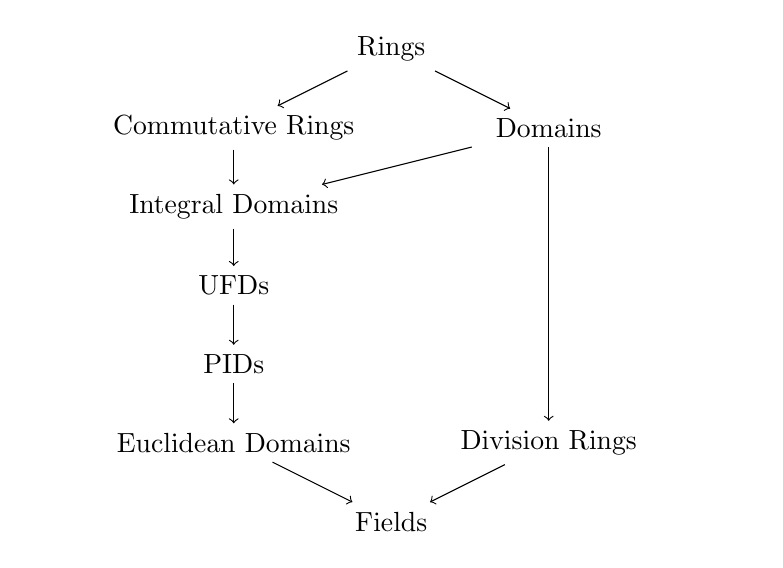
\begin{tikzpicture}[
      node distance=2cm,
      box/.style={
          text width=5cm,
          align=center
      }
      ]
      % Nodes for ring types
      \node[box] (rings) at (0,0) {Rings};
      \node[box] (comm) at (-2,-1) {Commutative Rings};
      \node[box] (domains) at (2,-1) {Domains};
      \node[box] (int) at (-2,-2) {Integral Domains};
      \node[box] (ufd) at (-2,-3) {UFDs}; % Added UFD between ID and PID
      \node[box] (divring) at (2,-5) {Division Rings};
      \node[box] (pid) at (-2,-4) {PIDs}; % Moved PID down
      \node[box] (euc) at (-2,-5) {Euclidean Domains}; % Moved ED down
      \node[box] (fields) at (0,-6) {Fields}; % Moved Fields down
      
      % Left path arrows
      \draw[->] (rings) -- (comm);
      \draw[->] (comm) -- (int);
      \draw[->] (int) -- (ufd); % New arrow to UFD
      \draw[->] (ufd) -- (pid); % New arrow from UFD to PID
      \draw[->] (pid) -- (euc);
      \draw[->] (euc) -- (fields);
      \draw[->] (divring) -- (fields);
      
      % Right path arrows
      \draw[->] (rings) -- (domains);
      \draw[->] (domains) -- (int);
      \draw[->] (domains) -- (divring);
    \end{tikzpicture}
    \caption{Basic hierarchy of rings with UFDs included.} 
    \label{fig:ring_hierarchy}
  \end{figure}

  Since a ring is a group with respect to addition, we know from \ref{thm:unique_add_inverse} that additive inverses are unique. However, we can say a little more with rings because of the distributive property. 

  \begin{lemma}[Additive Inverses] 
    Let $R$ be a ring. Then, for all $a, b \in R$, 
    \begin{enumerate}
      \item $0a = a0 = 0$. 
      \item $(-a)b = a(-b) = -(ab)$. 
      \item $(-a)(-b) = ab$. 
      \item The identity $1$ is unique and $-a = (-1)a$. 
    \end{enumerate}
  \end{lemma}
  \begin{proof}
    We can see that 
    \begin{align}
      -1 + 1 = 0 & \implies (-1 + 1) \times a = 0 \times a \\
    \end{align}
    and therefore by definition $-1 \times a$ must be the additive inverse. 
  \end{proof} 

  We will provide some examples of rings, though we have not properly defined some of them yet. We have only properly defined the power set ring and the integer ring in set theory. As for the rest, I hope the reader is familiar enough with these materials to at least recognize that they are rings. 

  \begin{example}[Power Set]
    Given a set $X$, $(2^X, \bigtriangleup, \cap)$ is a commutative associative ring with respect to the operations of symmetric difference $M \bigtriangleup N \coloneqq (M \setminus N) \cup (N \setminus M)$ and intersection. The additive identity is $\emptyset$ and the multiplicative identity is $X$. We can clearly see that both operations are commutative and $\cap$ is associative. 
    \begin{align*}
      M \bigtriangleup N & = (M \setminus N) \cup (N \setminus M) \equiv N \bigtriangleup M \\
      M \cap N & = N \cap M \\
      M \cap N \cap P & = (M \cap N) \cap P = M \cap (N \cap P)
    \end{align*}
  \end{example}

  \begin{example}[Number Systems]
    $(\mathbb{Z}, +, \times)$, $(\mathbb{Q}, +, \times)$, $(\mathbb{R}, +, \times)$, $(\mathbb{C}, +, \times)$ are all commutative rings, with additive and multiplicative identities $0$ and $1$. 
  \end{example}

  \begin{example}[Matrix Rings]
    The set of matrices $\mathbb{R}^{n \times n}$\footnote{really over any field and even more generally a ring $R$} forms a noncommutative ring under matrix addition $+$ and multiplication $\times$. It has the additive and multiplicative identities $0$ and $I_{n}$. This forms a non-commutative ring for $n > 1$, even when $R$ is commutative.
  \end{example}

  \begin{example}[Polynomials]
    The set of all polynomials over the reals are a ring. 
  \end{example}

  \begin{example}[Continuous Functions]
    The set of all continuous functions $f: \mathbb{R} \rightarrow \mathbb{R}$ is a ring under point-wise addition and multiplication. 
  \end{example}

  Next, just like how we did for groups, we can talk about subrings. 

  \begin{definition}[Subring]
    Given ring $(R, +, \times)$ a \textbf{subring} $(S, +, \times)$ is a ring such that $S \subset R$. $S$ is called a \textbf{proper subring} if $S \subsetneq R$. 
  \end{definition}

  \begin{example}[Quadratic Field]
    Let $D \in \mathbb{Q}$ be a square-free rational number (as in $D$ cannot be expressed as the perfect square of another rational). Now let us consider the set 
    \begin{equation}
      \mathbb{Q} (\sqrt{D}) \coloneqq \{a + b \sqrt{D} \mid a, b \in \mathbb{Q} \}
    \end{equation}
    equipped with component-wise addition and multiplication where $\sqrt{D}^2 = D$ and the rational commute with $\sqrt{D}$. This is indeed a commutative subring of $\mathbb{R}$. 
  \end{example}

  \begin{example}[Gaussian Integers]
    The \textbf{Gaussian integers} is the set 
    \begin{equation}
      \mathbb{Z}[i] \coloneqq \{a + bi \mid a, b \in \mathbb{Z} \} \subset \mathbb{C}
    \end{equation}
    equipped with component-wise addition and multiplication where $i^2 = 1$ and reals commute with $i$. This is indeed a commutative subring of $\mathbb{C}$. 
  \end{example}

  \begin{theorem}[Intersections of Subrings is a Subring]
    If $S_1, S_2$ are subrings of $R$, then $S_1 \cap S_2$ is a subring. 
  \end{theorem}

  Finally, we will mention a product ring. 

  \begin{definition}[Direct Product of Rings]
    Given rings $(R, +_R, \times_R)$ and $(S, +_S, \times_S)$, the direct product of the rings is the set $R \times S$ with the operations 
    \begin{enumerate}
      \item $(r_1, s_1) + (r_2, s_2) \coloneqq (r_1 +_R r_2, s_1 +_S s_2)$. 
      \item $(r_1, s_1) \times (r_2, s_2) \coloneqq (r_1 \times_R r_2, s_1 \times_S s_2)$. 
    \end{enumerate}
  \end{definition}
  \begin{proof}
    The proof is standard. 
  \end{proof}

\subsection{Ring Homomorphisms}

  So far, we have talked about many properties of rings but have not thoroughly gone over their classification. This is what we will do in this section, just like how we have classified groups. It turns out that classifying rings is significantly harder to do so, so we will talk about some low-order finite rings and provide some examples of isomorphisms between more complex rings. 

  \begin{definition}[Ring Homomorphism, Isomorphism]
    A \textbf{ring homomorphism} $f: R \rightarrow S$ is a function that satisfies for all $a, b \in R$
    \begin{enumerate}
      \item $f(a + b) = f(a) + f(b)$
      \item $f(ab) = f(a) f(b)$ 
      \item $f(1_R) = 1_S$\footnote{The reason we need this third is that while $f$ is a group homomorphism with respect to $+$, it automatically follows that $f(0) = 0$. However $f$ is only a monoid homomorphism w.r.t. $\times$, and so we need this extra constraint. }
    \end{enumerate}
    for all $a, b \in R$.\footnote{Note that the first is equivalent to it being a group homomorphism between $(R, +)$ and $(S, +)$. The second property may look like it is a group homomorphism between $(R, \times)$ and $(S, \times)$, but remember that neither are groups and it just states that closure distributes. Combined with the fact that the multiplicative identity matches, $f$ is really a homomorphism of \textit{monoids}. } Furthermore, 
    \begin{enumerate}
      \item A \textbf{ring isomorphism} is a bijective ring homomorphism, and we call rings $R$ and $S$ isomorphic, denoted $R \simeq S$ if there exists an isomorphism between them. 
      \item A \textbf{ring endomorphism} is a ring homomorphism onto itself. 
      \item A \textbf{ring automorphism} is an isomorphism from a ring to itself. 
    \end{enumerate}
  \end{definition} 

  \begin{example}[Homomorphisms of Rings]
    We provide some simple examples of ring homomorphisms. 
    \begin{enumerate}
      \item The identity map $\iota : R \to R$ is a ring automorphism. 
      \item If $R \subset S$ as rings, then the canonical injection map $\iota: R \to S$ is a ring homomorphism. 
      \item Complex conjugation $z \in \mathbb{C} \mapsto \bar{z} \in \mathbb{C}$ is a ring automorphism. 
      \item Differentiation is a ring automorphism over the polynomial ring $\mathbb{R}[x]$. 
    \end{enumerate}
  \end{example} 

  \begin{definition}[Kernel]
    The \textbf{kernel} of a ring homomorphism $f: R \rightarrow S$ is the preimage of $0 \in S$.\footnote{Note that this is the additive identity, not the multiplicative identity. We must specify which identity, unlike a group which has just one identity.}
  \end{definition}

  \begin{lemma}[Images and Kernels of Ring Homomorphisms]
    If $f: R \rightarrow S$ is a ring homomorphism, then 
    \begin{enumerate}
      \item $\im{f}$ is a subring of $S$. 
      \item $f$ is injective iff $\ker{f} = \{0\}$. 
    \end{enumerate}
  \end{lemma}
  \begin{proof}
    For the first claim, let $x, y, z \in \im{f}$. Then $x = f(a), y = f(b), z = f(c)$ for some $a, b \in R$. 
    \begin{enumerate}
      \item \textit{Closed under Addition}. $x + y = f(a) + f(b) = f(a + b) \in \im{f}$. 
      \item \textit{Associative under Addition}. $(x + y) + z = f(a + b) + f(c) = f((a + b) + c) = f(a + (b + c)) = f(a) + f(b + c) = x + (y + z)$
      \item \textit{Additive Identity}. $f(0) = 0$
      \item \textit{Additive Inverses}. We claim that $x^{-1} = f(a)^{-1} = f(a^{-1})$. Indeed, we have $f(a) f(a^{-1}) = f(a a^{-1}) = f(1) = 1$. 
      \item \textit{Closed under Multiplication}. $xy = f(a) f(b) = f(ab) \in \im{f}$. 
      \item \textit{Multiplicative Identity}. $f(1) = 1$. 
    \end{enumerate}
    For the second claim, we prove bidirectionally. 
    \begin{enumerate}
      \item $(\rightarrow)$. Let $\ker{f} \neq \{0\}$ and call its nonzero element $k$. Then, $f(a + k) = f(a) + f(k) = f(a) + 0 = f(a)$, and so $f(a) = f(a + k)$, which means $f$ is not injective. 
      \item $(\leftarrow)$. Assume that $f$ is not injective. Then there exists $a, b \in R$ s.t. $f(a) = f(b)$. This means that $0 = f(a) - f(b) = f(a - b)$, and so $a - b \in \ker{f}$. 
    \end{enumerate}
  \end{proof}

  Note that $\ker{f}$ is \textit{not} a subring, and we can quickly verify this by noticing that the identity element does not necessarily have to be in the kernel. However, we will see later that this is a specific instance of a more general structure called an \textit{ideal}. 

  \begin{theorem}[Compositions of Ring Homomorphisms]
    Compositions of ring homomorphisms are ring homomorphisms. 
  \end{theorem} 
  \begin{proof}
    Let $R \xrightarrow{f} S \xrightarrow{g} T$ be two ring homomorphisms. We can see that 
    \begin{enumerate}
      \item $(g \circ f)(a + b) = g( f(a) + f(b)) = g(f(a)) + g(f(b))$. 
      \item $g(f(ab)) = g(f(a) f(b)) = g(f(a)) + g(f(b))$ 
      \item $g(f(1_R)) = g(1_S) = 1_T$
    \end{enumerate}
  \end{proof}

  Now let's focus a bit more on ring isomorphisms. The following should be intuitive. 

  \begin{lemma}[Inverse of Ring Isomorphism is an Isomorphism]
    If $f: R \to S$ is a ring isomorphism, then $f^{-1}$ is a ring isomorphism. 
  \end{lemma} 
  \begin{proof}
    Since $f$ is a bijection, $f^{-1}$ is well defined and is a bijection. Now let $x, y \in S$, which implies that $x = f(a), y = f(b)$ for a unique $a, b \in R$. Now we see that $f^{-1}$ satisfies the 3 properties of a ring homomorphism. 
    \begin{enumerate}
      \item $f^{-1} (x + y) = f^{-1} (f(a) + f(b)) = f^{-1}(f(a + b)) = a + b = f^{-1}(a) + f^{-1} (b)$. 
      \item $f^{-1} (x y) = f^{-1} (f(a) f(b)) = f^{-1}(f(a b)) = a b = f^{-1}(a) f^{-1} (b)$. 
      \item $f^{-1}(1_S) = 1_R$. 
    \end{enumerate}
    Therefore, as a bijective ring homomorphism $f^{-1}$ is also a ring isomorphism. 
  \end{proof}

\subsection{Characteristics}

  Note that given a ring $R$, we can pay attention to the subring $\langle 1 \rangle$. This must either be isomorphic to $\mathbb{Z}$ or $\mathbb{Z}_n$, so we can think of it being embedded in $R$. 
  
  \begin{theorem}[Integer Ring Exists in Any Ring]
    For every ring $R$, there exists a unique ring homomorphism $f: \mathbb{Z} \to R$. 
  \end{theorem}
  \begin{proof}
    We know that $f(1_{\mathbb{Z}}) = 1_R$, and so for $n > 0$, 
    \begin{align}
      f(n_{\mathbb{Z}}) & = f(1_{\mathbb{Z}} + \ldots + 1_{\mathbb{Z}}) \\
                        & = f(1_{\mathbb{Z}}) + \ldots + f(1_{\mathbb{Z}}) \\
                        & = 1_R + \ldots + 1_R \\
                        & = n_R
    \end{align} 
    Similarly, we have 
    \begin{align}
      f(-n_{\mathbb{Z}}) & = f(-1_{\mathbb{Z}} - \ldots - 1_{\mathbb{Z}}) \\
                         & = f(1_{\mathbb{Z}}) - \ldots - f(1_{\mathbb{Z}}) \\
                         & = -1_R - \ldots - 1_R \\
                         & = -n_R
    \end{align} 
    Since $\mathbb{Z}$ is a PID, $\ker{f}$---which is an ideal---must be principal, and so $\ker{f} = \langle m \rangle$ for some $m \in \mathbb{Z}$. 
  \end{proof} 

  Therefore, this motivates the following attribute of a ring, i.e. the smallest $\langle m \rangle$ that embeds (an injective homomorphism) into the ring. 

  \begin{definition}[Characteristic Number]
    The \textbf{characteristic} of ring $R$, denoted $\Char(R)$, is defined equivalently. 
    \begin{enumerate}
      \item It is the smallest number of times one must successively add the multiplicative identity $1$ to get the additive identity $0$. 
      \begin{equation}
        1 + 1 + ... + 1 = 0 
      \end{equation}
      If no such number $n$ exists, then $\Char(R) = 0$. 

    \item It is equal to $m$, where $\ker{f} = \langle m \rangle$ for the homomorphism defined above.\footnote{Note that $m$ always exists since $\mathbb{Z}$ is a PID.}
    \end{enumerate}
  \end{definition}

  Often, it is not obvious whether two given rings $R$ and $S$ are isomorphic. The characteristic number is preserved across ring isomorphisms and therefore is a good sanity check. 

  \begin{theorem}[Preservation of Characteristic Number in a Ring Homomorphism]
    $R \simeq S \implies \Char(R) = \Char(S)$. 
  \end{theorem}
  \begin{proof}

  \end{proof}

  However, the converse is not true! If so, we would have completely classified all rings just based on their characteristic number, and the study of rings would end pretty soon. 

  \begin{example}[Same Characteristic does not Imply Isomorphic]
    There exists no isomorphism from $\mathbb{Z}$ to $\mathbb{R}$. 
  \end{example}

  \begin{theorem}[Wilson's Theorem]
    Let $p \in \mathbb{N}$ be prime. Then 
    \begin{equation}
      (p-1)! \equiv -1 \pmod{p}
    \end{equation}
  \end{theorem}
  
\subsection{Divisors and Reducibility} 

  Note that we do not assume that there exists multiplicative inverses in a ring. However, there may be some elements for which multiplicative inverses do exist, i.e. $a, b \in R$ where $ab = 1$. 

  \begin{definition}[Unit]
    A \textbf{unit} of a ring $R$ is an element $u \in R$ that has a multiplicative inverse in $R$. That is, there exists a $v \in R$ s.t. $uv = vu = 1$. 
  \end{definition}

  \begin{example}[Units and Non-Units]
    A ring $R$ may have either none (except for $0$ and $1$), some, or all of its elements as units. 
    \begin{enumerate}
      \item $\mathbb{Z}$ has no non-unity element that is a unit. For example, given $z \in \mathbb{Z}$, there is no element of the form $1/z$.  
      \item In $\mathbb{Q}$, every nonzero element is a unit. Given any element of form $\frac{p}{q} \in \mathbb{Q}$, the element $\frac{q}{p}$ is the multiplicative inverse. 
      \item In $\mathbb{Z}_8$, the units are $1, 3, 5, 7$ as $1 \cdot 1 = 3 \cdot 3 = 5 \cdot 5 = 7 \cdot 7 = 1$. However, $0, 2, 4, 6$ are not units since you can look in $\mod{2}$. 
    \end{enumerate}
  \end{example}

  Another property that we would desire is some sort of decomposition of ring elements as other ring elements. More specifically, the existence of elements $a, b$ such that $ab = 0$ will be of particular interest to us. 

  \begin{definition}[Left, Right Divisor]
    Let $a, b, r \in R$ a ring. 
    \begin{enumerate}
      \item If $ab = r$, then $a$ is said to be a \textbf{left divisor} of $r$ and $b$ a \textbf{right divisor} of $r$. 

      \item $a$ is said to be a left divisor of $r$ if it is a left divisor and a right divisor of $r$: $ax = ya = r$, but $x$ does not necessarily equal $y$. 

      \item If $ab = 0$, then $a$ and $b$ are said to be a \textbf{left zero divisor} and \textbf{right zero divisor}, respectively. 
    \end{enumerate}
    If $R$ is commutative, then we just call $a$ a \textbf{divisor} of $r$ or a \textbf{zero divisor}.\footnote{$a$ is a right divisor of $b \iff \exists x (xa = b) \iff \exists x (ax = b) \iff a$ is a left divisor. } 
  \end{definition}

  \begin{definition}[Reducibility of Elements]
    Let $R$ be a commutative ring and $r \in R$ be nonzero and not a unit. 
    \begin{enumerate}
      \item Then $r$ is \textbf{irreducible} in $R$ if whenever $r = ab$ with $a, b \in R$, at least one of $a, b$ is a unit in $R$. 
      \item Otherwise, $r$ is said to be \textbf{reducible}, and $a, b$ are said to be \textbf{factors}
    \end{enumerate}
  \end{definition}
  
  Note that reducibility is slightly different than the existence of divisors of an element. $r$ may have divisors, but they could also be units. Therefore, irreducibility is weaker than having no divisors. This should not be mixed up with prime/composite elements either, which we have not defined 

  \begin{lemma}[Units and Zero Divisors are Mutually Exclusive]
    An element $a \in R$ can never be both a unit and a zero divisor. 
  \end{lemma}
  \begin{proof}
    Let $a \in R$ be a unit. Then $1 = ab$ for some $b \in R$. Now if $a$ was a zero divisor, then $ra = 0$ for some $r \in R$. However, we have $r(ab) = r1 = r \neq 0 = 0b = (ra)b$, which contradicts associativity. 
  \end{proof}

  Let's go through some examples to see that we can have widely differing behavior in terms of divisors. 

  \begin{example}[Left Divisor But Not Right Divisor in Matrix Ring]
    Let us define the ring
    \begin{equation}
      R = \begin{pmatrix} \mathbb{Z} & \mathbb{Z}_2 \\ 0 & \mathbb{Z} \end{pmatrix} = \bigg\{ \begin{pmatrix} x & y \\ & z \end{pmatrix} \; \bigg| \; x, z \in \mathbb{Z}, y \in \mathbb{Z}_2 \bigg\} 
    \end{equation}
    This should be checked that it is a ring. Let 
    \begin{equation}
      a = \begin{pmatrix} 2 & 0 \\ 0 & 1 \end{pmatrix}, \; b = \begin{pmatrix} 0 & 1 \\ 0 & 0 \end{pmatrix}
    \end{equation}
    Then, we can see that $ab = 0$ but $ba \neq 0$. That is, $b$ is a right zero divisor of $a$, but $b$ is not a left zero divisor. 
  \end{example}

  Note that $0$ is divisible by every element since $0a = 0$ for all $a \in R$. Furthermore, if $p$ was a unit, then it can always be multiplied by $p^{-1}$ and then by any $a \in R$ to get the factorization $a = (a p^{-1}) p$. So $p$ as a unit would divide \textit{every} element in $R$. 

  \begin{example}[Prime and Composite Elements]
    An element in a ring $R$ may either be prime, composite, or neither. 
    \begin{enumerate}
      \item In $\mathbb{Z}$, $2$ is prime but $6 = 2 \cdot 3$. 
      \item In $\mathbb{Q}$, there are no such things are prime or composite elements since every nonzero element is a unit. 
      \item In $\mathbb{Z}_5$, every nonzero element is a unit since $2 \cdot 3 = 4 \cdot 4 = 1$, so calling the elements prime or composite does not make sense. 
      \item In $\mathbb{Z}_6$, $2, 4$ are not units, so they must be either prime or composite. It turns out that $2$ is prime and $4 = 2 \cdot 2$ is composite. 
    \end{enumerate}
  \end{example}

  Therefore, in a general ring there is too little structure to determine much about the divisibility of elements. The following lemma is all we have. 

  \begin{lemma}[Divisibility of Linear Combinations of Rings Elements]
    Let $R$ be a commutative ring and $a, b, d \in R$. If $d \mid a$ and $d \mid b$, then $d \mid (ma + nb)$ for any $m, n \in R$. 
  \end{lemma} 

  One may also intuit that when $a \mid b$, $a$ must be ``less than'' $b$. First, in a ring without an order or a norm, this statement doesn't really make sense, and you can indeed have two distinct elements that are divisors of each other! 

  \begin{example}[Two Distinct Elements are Divisors of Each Other]
    In $\mathbb{Z}_{12}$, we have 
    \begin{enumerate}
      \item $2 \mid 10$ since $10 = 2 \cdot 5$, and $10 \mid 2$ since $2 = 10 \cdot 5$. 
      \item $3 \mid 9$ since $9 = 3 \cdot 3$ and $3 \mid 9$ since $3 = 9 \cdot 7$. 
    \end{enumerate}
  \end{example}

  Therefore, this motivates the following definition. 

  \begin{definition}[Associate Elements]
    Elements $a$ and $b$ are \textbf{associated}, denoted $a \sim b$ if either of the following equivalent conditions holds
    \begin{enumerate}
      \item $a \mid b$ and $b \mid a$. 
      \item $a = u b$, for some unit $u \in R$. 
    \end{enumerate}
    This forms an equivalence relation. 
  \end{definition} 
  \begin{proof}
    We first prove the equivalence. 
    \begin{enumerate}
      \item Assume that $a \mid b$ and $b \mid a$. Then $a \mid b \implies b = ra$ for some $r \in R$. Furthermore, $b \mid a \implies a = qb$ for some $q \in R$. Therefore, we have $b = ra = (rq)b$, and so $rq = 1$, which means $r, q$ must be units. 
      \item Assume that $a = ub$ for some unit $u \in R$. Then, $b \mid a$. Now, we can multiply by $u^{-1}$ to get $u^{-1} a = b \implies a \mid b$. 
    \end{enumerate}
    To prove that this is an equivalence relation, we prove the following properties. 
    \begin{enumerate}
      \item \textit{Reflexive}. $a \sim a$ since $a = 1a$. 
      \item \textit{Symmetric}. If $a \sim b$, then $a \mid b$ and $b \mid a$, implying that $b \sim a$. 
      \item \textit{Transitive}. If $a \sim b, b \sim c$, then there exists units $u, v \in R$ s.t. $a = ub, b = vc$, and so $a = (uv)c$, where $uv$ is a unit with $(uv)^{-1} = v^{-1} u^{-1}$. 
    \end{enumerate}
  \end{proof}

  \begin{example}[Associate Elements in a Commutative Ring]
    We present some examples of associate elements. 
    \begin{enumerate}
      \item In $\mathbb{Z}$, $\pm 6$ are associate elements since $6 = -1 \cdot 6$, where $-1$ is a unit. 
      \item In $\mathbb{Z}[i]$, $1 + i$, $1 - i$ are associate elements since $1 + i = i (1 - i)$, where $i$ is a unit since $i \cdot -i = 1$. 
      \item As above, in $\mathbb{Z}_{12}$ the elements $2, 10$ are associate elements since $2 = 5 \cdot 10$, where $5$ is a unit since $5 \cdot 5 = 1$. 
    \end{enumerate}
  \end{example}

  Remember that for commutative rings, distinguishing left and right divisors are meaningless, and so we can talk about just \textit{divisors}. Almost all rings that we will deal with are commutative, so let's try to find some properties of commutative rings.  

  \begin{definition}[Greatest Common Divisor]
    Let $R$ be a commutative ring and let $a, b \in R$ with $b \neq 0$. The \textbf{greatest common divisor} of elements $a$ and $b$---denoted $\gcd(a, b)$---is an element $d \in R$ satisfying: 
    \begin{enumerate}
      \item $d \mid a$ and $d \mid b$ 
      \item if $k \mid a$ and $k \mid b$, then $k \mid d$. 
    \end{enumerate}
    If $\mathrm{gcd}(a, b) = 1$, then $a$ and $b$ are said to be \textbf{relatively prime}. 
  \end{definition} 

  Note that in an arbitrary commutative ring, the gcd of two elements always exists since we can at least identify $1$, but there may not be a \textit{unique} gcd. 

\subsection{Ideals}

  Now assuming that $R$ and $S$ are commutative rings, let's consider a special sort of subset of a commutative ring. Consider the kernel of the ring homomorphism. We can see that if $a, b \in \ker(f)$, then $f(a + b) = f(a) + f(b) = 0 + 0 = 0$, and so $\ker(f)$ is closed under addition. Furthermore, $a \in \ker(f)$ and \textit{any} $b \in R$ gives $f(ab) = f(a) f(b) = 0 f(b) = 0$, and so multiplying any element in the kernel by an arbitrary element in the rings keeps it in the kernel. We would like to generalize these properties into an \textit{ideal}. 

  \begin{definition}[Ideals]
    For a commutative ring $(R,+, \times)$, a \textbf{two-sided ideal}---or \textbf{ideal}---is a subset $I \subset R$ satisfying 
    \begin{enumerate}
      \item $a, b \in I \implies a + b \in I$. 
      \item $a \in I, r \in R \implies ra = ar \in I$.\footnote{Note that this property and closure under addition actually implies that it is an abelian subgroup under addition, since we can see that $-1 \in R$ and $a \in I$ implies $-1 \cdot a = -a \in I$.}
    \end{enumerate}
    If $R$ is not necessarily commutative, then we $ra \neq ar$ in general, so we may distinguish between left and right ideals. 
  \end{definition}

  Therefore, we can see that it is an abelian group under $+$ and closed under $\times$. However, it is not guaranteed to have a multiplicative identity, which is why we can interpret $I$ as a ring without a multiplicative identity, also known as a \textit{rung}. Ideals are analogous to normal subgroups, which were used to induce a congruence relation on a group to get its quotient. Ideals play a similar role. 

  \begin{example}[Matrix with Last Row of Zeros]
    Let $R$ be the set of all $n \times n$ matrices. Then 
    \begin{enumerate}
      \item The set of all $n \times n$ matrices whose last row is zero forms a right ideal, but not a left ideal.
      \item The set of all $n\times n$ matrices whose last column is zero is a left ideal, but not a right ideal. 
    \end{enumerate}
  \end{example}

  \begin{example}[Multiples of Elements Are an Ideal]
    We give 2 ideals: 
    \begin{enumerate}
      \item The set of even integers $2 \mathbb{Z}$ is an ideal in the ring $\mathbb{Z}$, since the sum of any even integers is even and the product of any even integer with an integer is an even integer. However, the odd integers do not form an ideal. 
      \item The set of all polynomials with real coefficients which are divisible by the polynomial $x^2 + 1$ is an ideal in the ring of all polynomials. 
    \end{enumerate}
  \end{example}

  Let's talk about a few more properties of ideals, namely their construction and behavior under set theoretic operations. 

  \begin{theorem}[Sum and Intersection of Ideals are Ideals] 
    \label{thm:sum_int_ideals}
    Given two ideals $I, J \subset R$, 
    \begin{enumerate}
      \item $I \cap J$ is an ideal. 
      \item $I + J \coloneqq \{i + j \mid i \in I, j \in J\}$ is an ideal. 
    \end{enumerate}
  \end{theorem}
  \begin{proof}
    Listed. 
    \begin{enumerate}
      \item $I \cap J$ is an ideal. Given $a, b \in I \cap J$, then $a, b \in I \implies a + b \in I$, and $a, b \in J \implies a + b \in J$. So $a + b \in I \cap J$. Furthermore, for every $r \in R$, $a \in I \implies r a \in I$ and $a \in J \implies r a \in J$, so $a \in I \cap J \implies ra \in I \cap J$. 

      \item $I + J$ is an ideal. Given $x, y \in I + J$, then $x = a_x + b_x$ and $y = a_y + b_y$ for $a_x, a_y \in I, b_x, b_y \in J$. So 
      \begin{equation}
        x + y = (a_x + b_x) + (a_y + b_y) = (a_x + a_y) + (b_x + b_y)
      \end{equation}
      where $a_x + a_y \in I, b_x + b_y \in J$ by definition of an ideal, and so $x + y \in I + J$. Noe let $x = a_x + b_x \in I + J$. Then given $r \in R$,
      \begin{equation}
        rx = r(a_x + b_x) = r a_x + r b_x
      \end{equation}
      where $r a_x \in I$ and $r b_x \in J$ since $I, J$ are ideals. Therefore $rx \in I + J$.  
    \end{enumerate}
  \end{proof}
  
  \begin{theorem}[Preimage of Ideals are Ideals]
    If $f: R \to S$ is a ring homomorphism of commutative rings $J \subset S$ is an ideal, then $f^{-1} (J)$ is an ideal of $R$. 
  \end{theorem}
  \begin{proof}
    We prove the two properties of an ideal. 
    \begin{enumerate}
      \item Consider $a, b \in f^{-1} (J) \subset R$. Then $f(a + b) = f(a) + f(b) \in J \implies a + b \in f^{-1}(J)$. 
      \item Consider $r \in R$ and $a \in I f^{-1}(J)$. Then, $f(ra) = f(r) f(a)$ where $f(r) \in S$ and $f(a) \in J$. So $f(r) f(a) = f(ra) \in J \implies ra \in f^{-1}(J)$. 
    \end{enumerate}
  \end{proof}

  \begin{example}[Image of Ideal is Not Necessarily an Ideal]
    It is not true in general that for an ideal $I \subset R$ and a ring homomorphism $f: R \to S$, the image $f(I)$ is an ideal of $S$. 
  \end{example}

  Given the two examples above, let's formalize the idea of an ideal consisting of all multiples of a specific element $a$. This sounds pretty familiar to \textit{generators} of groups. 

  \begin{definition}[Generators of Ideals]
    Given a commutative ring $R$, the \textbf{ideal generated by $a \in R$} is denoted 
    \begin{equation}
      \langle a \rangle \coloneqq \{r a \mid r \in R\}
    \end{equation}
    and more generally, we may have multiple generating elements. 
    \begin{equation}
      \langle a_1, \ldots, a_n \rangle \coloneqq \{ r_1 a_1 + \ldots r_n a_n \mid r_1, \ldots, r_n \in R \}
    \end{equation}
  \end{definition}

  A good---yet not completely accurate---intuition to have about ideals is that they are the set of multiples of a certain element. This technically isn't true in general, but if this intuition is true, then we call this a \textit{principal ideal}. 

  \begin{definition}[Principal Ideals]
    A \textbf{principal ideal} is an ideal generated by a single element: $I = \langle a \rangle$. 
  \end{definition}

  \begin{example}[Some Principal Ideals]
    Let's take a look at some examples and non-examples of principal ideals. 
    \begin{enumerate}
      \item In any ring $R$, the sets $\{0\} = \langle 0 \rangle$ and $R$ are principal ideals. 
      \item The set of all even integers $2\mathbb{Z} = \{\ldots, -4, -2, 0, 2, 4, \ldots\}$ is a principal ideal generated by $2 \in \mathbb{Z}$. 
      \item The set of all imaginary multiples $i\mathbb{Z} = \{ai \mid a \in \mathbb{Z} \}$ is a principal ideal $\langle i \rangle \subset \mathbb{Z}[i]$. 
    \end{enumerate}
  \end{example}

  What is nice about principal ideals it that they ``encode'' the divisors. 

  \begin{theorem}[Principal Ideals and Divisors]
    Given a commutative ring $R$ and $a, b \in R$, the following are equivalent. 
    \begin{enumerate}
      \item $b \mid a$. 
      \item $a \in \langle b \rangle$. 
      \item $\langle a \rangle \subset \langle b \rangle$. 
    \end{enumerate}
  \end{theorem}
  \begin{proof}
    
  \end{proof}

  This allows us to define the GCD with ideals. 

  \begin{corollary}[GCD as a Minimal Ideal]
    Let $R$ be a commutative ring, $a, b \in R$, and $I = \langle a, b \rangle$. Then $d$ is the greatest common divisor if 
    \begin{enumerate}
      \item $I$ is contained in the principal ideal $\langle d \rangle$. 
      \item If $\langle d^\prime \rangle$ is any principal ideal containing $I$, then $\langle d \rangle \subseteq \langle d^\prime \rangle$. 
    \end{enumerate}
  \end{corollary}
  \begin{proof}
    
  \end{proof}

  That is, a greatest common divisor of $a, b$ is a generator for the smallest principal ideal containing $a$ and $b$. However, there are cases in which the gcd is not unique, and hence there are multiple elements $d, d^\prime$ that generate such a minimal ideal! This can happen in two ways: either $\langle d \rangle = \langle d^\prime \rangle$, or both principal ideals $\langle d \rangle, \langle d^\prime \rangle$ contain $a$ and $b$ but are not contained in each other. 

  \begin{example}[Two Distinct Elements can Generate the Same Ideal]
    Continuing on our example from before, let's verify that the associate elements indeed generate the same ideal. 
    \begin{enumerate}
      \item For $\pm 6 \in \mathbb{Z}$, we indeed have 
        \begin{align}
          \langle 6 \rangle & = \{ \ldots, -12, -6, 0, 6, 12, \ldots \} \\
          \langle -6 \rangle & = \{ \ldots, 12, 6, 0, -6, -12, \ldots \} 
        \end{align}

      \item For $1 + i, 1 - i \in \mathbb{Z}[i]$, every element in $\langle 1 + i \rangle$ is of the form $r (1 + i)$ for some $r \in \mathbb{Z}[i]$. Therefore, 
        \begin{equation}
          r(1 + i) = ri (-i)(1 + i) = ri (1 - i) \in \langle 1 - i \rangle
        \end{equation}
        for some $ri \in \mathbb{Z}[i]$, implying that $\langle 1 + i \rangle \subset \langle 1 - i \rangle$. The reverse inclusion is the same logic. 

      \item Given $2, 10 \in \mathbb{Z}_{12}$, let us write out their ideals. 
        \begin{align}
          \langle 2 \rangle & = \{0, 2, 4, 6, 8, 10\} \\ 
          \langle 10 \rangle & = \{0, 10, 20 = 8, 18 = 6, 16 = 4, 14 = 2\}
        \end{align}
    \end{enumerate}
  \end{example} 

  This gives us a hint as to what these elements are. 

  \begin{theorem}[Elements that Generate Same Ideal are Associated]
    Given commutative ring $R$ and $a, b \in R$, $a$ and $b$ are associate elements if and only if $\langle a \rangle = \langle b \rangle$. 
  \end{theorem}
  \begin{proof}
    We prove bidirectionally. 
    \begin{enumerate}
      \item $(\rightarrow)$. Let $a, b \in R$ be associate elements. Then there exists a unit $u \in R$ s.t. $a = ub$. Therefore $ \langle a \rangle \subset \langle b \rangle$. On the other hand, $b = u^{-1} a$, and so $\langle b \rangle \subset \langle a \rangle$. 
      \item $(\leftarrow)$. Let $\langle a \rangle = \langle b \rangle$. Then this implies that $a \mid b$ and $b \mid a$, and so they are associate elements. 
    \end{enumerate}
  \end{proof}

  Now that we have learned ideals, we can define prime ideals and prime elements. 
  
  \begin{definition}[Prime Ideal]
    An ideal $P$ of a commutative ring $R$ is \textbf{prime} if it has the following two properties. 
    \begin{enumerate}
      \item If $a, b \in R$ where $ab \in P$, then either $a \in P$ or $b \in P$. 
      \item $P \subsetneq R$. 
    \end{enumerate}
  \end{definition}

  \begin{definition}[Prime Elements]
    Let $R$ be a commutative ring and $p \in R$ be nonzero and not a unit. $p$ is \textbf{prime} if either of the equivalent conditions is true. 
    \begin{enumerate}
      \item The ideal $\langle p \rangle$ is a prime ideal. 
      \item Whenever $p \mid ab$ for any $a, b \in R$, then either $p \mid a$ or $p \mid b$. 
    \end{enumerate}
  \end{definition}

  The final property of ideals is whether it ``almost'' fills up the whole ring in that it is maximal. 

  \begin{definition}[Maximal Ideal]
    Let $R$ be a commutative ring and $I \subset R$ an ideal. $I$ is \textbf{maximal} if there exists no ideal $J$ s.t. $I \subsetneq J \subsetneq R$. 
  \end{definition}

\subsection{Quotient Rings}

  What is nice about ideals is that they induce not just an equivalence relation---but a congruence relation---on a ring, which is a generalization of working in the integers modulo $n$. 

  \begin{theorem}[Equivalence Relation Induced by an Ideal]
    Given a commutative ring $R$ and an ideal $I \subset R$, we say that two elements $a, b \in R$ are \textbf{congruent} $\pmod{I}$, written $a \equiv b \pmod{I}$ iff $a - b \in I$. We claim two things: 
    \begin{enumerate}
      \item $\equiv$ is an equivalence relation. 
      \item $\equiv$ is a congruence relation. Given that $a \equiv a^\prime \pmod{I}$ and $b \equiv b^\prime \pmod{I}$, 
      \begin{equation}
        a + b \equiv a^\prime + b^\prime \pmod{I}, \qquad ab \equiv a^\prime b^\prime \pmod{I}
      \end{equation}
    \end{enumerate}
    Occasionally, if the ideal $I$ is clear from context, we will write $a \equiv b$. 
  \end{theorem}
  \begin{proof}
    We first prove that $\equiv$ is indeed an equivalence relation. 
    \begin{enumerate}
      \item \textit{Reflexive}. $a \equiv a \pmod{I}$ is trivial since $a - a = 0 \in I$. 
      \item \textit{Symmetric}. If $a \equiv b$, then $a - b \in I \implies -(a - b) = -a + b = b - a \in I \implies b \equiv a$. 
      \item \textit{Transitive}. If $a \equiv b$ and $b \equiv c$, then $a - b \in I$ and $b - c \in I$. Since $I$ is an additive group and so it is closed under addition, so $(a - b) + (b - c) = a - c \in I \implies a \equiv c$. 
    \end{enumerate}
    Note that so far, we have only used the group property of ideals to prove that is is an equivalence class. Now for congruence of multiplication, we need the ring properties. 
    \begin{enumerate}
      \item $a \equiv a^\prime, b \equiv b^\prime \implies (a - a^\prime), (b - b^\prime) \in I$. By adding them together and distributivity, we have 
      \begin{equation}
        a - a^\prime + b - b^\prime = (a + b) - (a^\prime + b^\prime) \in I \implies a + b \equiv a^\prime + b^\prime \pmod{I}
      \end{equation}

      \item We see that $a \in R, (b - b^\prime) \in I \implies a(b - b^\prime) \in I$. Similarly, $b^\prime \in R, (a - a^\prime) \in I \implies (a - a^\prime) b^\prime \in I$. Now adding the two, we have 
      \begin{equation}
        a (b - b^\prime) + (a - a^\prime) b^\prime = ab - ab^\prime + ab^\prime - a^\prime b^\prime = ab - a^\prime b^\prime \in I \implies ab = a^\prime b^\prime \pmod{I}
      \end{equation}
    \end{enumerate}
  \end{proof} 

  This quotient space maintains a lot of nice properties of the algebraic operations, and so we can form a new ring structure with this quotient space.  

  \begin{definition}[Quotient Rings, Rings of Residue Class]
    The quotient space $R/I$ induced by the mapping $a \mapsto [a]$ is indeed a commutative ring, called the \textbf{quotient ring}, with addition and multiplication defined 
    \begin{equation}
      [a] + [b] \coloneqq [a + b], \qquad [ab] \coloneqq [a] \, [b]
    \end{equation}
  \end{definition}
  \begin{proof}
    Note that the properties of the operation in $\frac{M}{R}$ inherits all the properties of the addition operation on $M$ that are expressed in the form of identities and inverses, along with the existence of the zero identity. 
    \begin{align*}
      0 \in M & \implies [0] \text{ is the additive identity in } \frac{M}{R} \\
      a + (-a) = 0 & \implies [a] + [-a] = [0] \\
      1 \in M & \implies [1] \text{ is the multiplicative identity in } \frac{M}{R}
    \end{align*}
  \end{proof} 

  \begin{theorem}[Quotient Maps are Homomorphisms]
    The map $p: R \to R/I$ is a ring homomorphism. 
  \end{theorem}
  \begin{proof}
    This is true by definition since we have made $\equiv$ a congruence relation. 
  \end{proof}

  \begin{example}[Quotient Rings of Integers]
    The quotient set $\mathbb{Z}/\langle n \rangle$ by the relation of congruence modulo $n$ is denoted $\mathbb{Z}_{n}$. 
    \begin{equation}
      \mathbb{Z}_{n} = \{ [0]_{n}, [1]_{n}, \ldots, [n-1]_{n} \}
    \end{equation}
    Note that the quotient ring $(\mathbb{Z}/\langle n \rangle, +, \times)$ is precisely the cyclic quotient group $\mathbb{Z}_n = \mathbb{Z}/6\mathbb{Z}$ when considering only addition. We list some quotient rings of the integers. 
    \begin{enumerate}
      \item In $\mathbb{Z}_{5} = \mathbb{Z}/\langle 5 \rangle$, the elements $[2]$ and $[3]$ are multiplicative inverses of each other since $[2] [3] = [6] = [1]$, and $[4]$ is its own inverse since $[4] [4] = [16] = [1]$. The addition and multiplication tables for $\mathbb{Z}_5$ is shown below. 
      \item Consider the ideal $I = \langle 2 \rangle \subset \mathbb{Z}_6$. We have $0 \equiv 2 \equiv 4 \pmod{I}$ and $1 \equiv 3 \equiv 5 \pmod{I}$, and so the quotient ring $\mathbb{Z}_6 / I$ consists of the two equivalence classes $[0]$ and $[1]$. 
    \end{enumerate}
  \end{example}

  \begin{example}[Quotient Rings of Polynomials]
    We list some quotient rings of polynomials. 
    \begin{enumerate}
      \item Consider $\mathbb{Q}[x] / \langle x^2 - 2 \rangle$. We can see that any polynomial $f \in \mathbb{Q}[x]$ is equivalent $\pmod{I}$ to a linear polynomial, since $x^2 \equiv 2$. Alternatively we can apply the division algorithm to replace $f(x)$ by its remainder upon division by $x^2 - 2$, and thus in the quotient ring, $[x]$ plays the role of $\sqrt{2}$, which may indicate that $\mathbb{Q}[x] / \langle x^2 - 2 \rangle = \mathbb{Q}[\sqrt{2}]$. 
      \item Consider $\mathbb{Z}_2 [x]/ \langle x^2 + x + 1 \rangle$. As in the previous example, any polynomial in $\mathbb{Z}_2[x]$ is equivalent to a linear polynomial since $x^2 \equiv x + 1 \pmod{I}$. Therefore the elements of the quotient ring are $[0], [1], [x], [x+1]$ with the addition and multiplication tables. 

      \begin{figure}[H]
        \centering
        \begin{subfigure}[b]{0.48\textwidth}
          \centering
          \begin{tabular}{c|cccc}
            $+$ & $0$ & $1$ & $x$ & $x + 1$ \\
            \hline
            $0$ & $0$ & $1$ & $x$ & $x + 1$ \\
            $1$ & $1$ & $0$ & $x + 1$ & $x$ \\
            $x$ & $x$ & $x + 1$ & $0$ & $1$ \\
            $x + 1$ & $x + 1$ & $x$ & $1$ & $0$ \\
          \end{tabular}
          \caption{}
        \end{subfigure}
        \hfill 
        \begin{subfigure}[b]{0.48\textwidth}
          \centering
          \begin{tabular}{c|cccc}
            $\cdot$ & $0$ & $1$ & $x$ & $x + 1$ \\
            \hline
            $0$ & $0$ & $0$ & $0$ & $0$ \\
            $1$ & $0$ & $1$ & $x$ & $x + 1$ \\
            $x$ & $0$ & $x$ & $x + 1$ & $1$ \\
            $x + 1$ & $0$ & $x + 1$ & $1$ & $x$ \\
          \end{tabular}
          \caption{}
        \end{subfigure}
        \label{fig:boolean-algebra-tables}
      \end{figure}
    \end{enumerate}
  \end{example}

  Note that just like how quotient topologies do not preserve topological properties, as shown \hyperref[pst-quotient_trivial]{here} and \hyperref[pst-quotient_hausdorff]{here}, quotient rings inherit some---but not all---ring properties. It obviously inherits commutativity since the quotient space is constructed with a congruence relation. However, the characteristic is changed. 

  Just like in group theory, we have a method of constructing isomorphisms between cleverly chosen rings $S$ and a quotient ring $R/I$. This seems to be a common pattern here when considering groups, rings, and topological spaces... This will be investigated more in category theory. 

  \begin{theorem}[First Isomorphism Theorem for Rings]
    Let $R$ and $S$ be commutative rings, and suppose $f: R \rightarrow S$ be a surjective ring homomorphism. Then this induces a ring isomorphism
    \begin{equation}
      R /\ker{f} \simeq S
    \end{equation} 
    satisfying $\phi = \bar{\phi} \circ \pi$. 

    \begin{figure}[H]
      \centering 
      \begin{tikzcd}
        R \arrow[r, "\phi"] \arrow[d, "\pi"] & S \\
        R/\ker(\phi) \arrow[ru, "\bar{\phi}"] &  
      \end{tikzcd}
      \caption{The theorem states that the following diagram commutes. } 
      \label{fig:fund_ring_homo_theorem}
    \end{figure}
  \end{theorem}
  \begin{proof}
    
  \end{proof} 

  A direct application of this is the Chinese remainder theorem. 

  \begin{corollary}[Chinese Remainder Theorem]
    Given a commutative ring $R$, let $I, J \subset R$ be ideals such that $I + J = R$. Then, 
    \begin{equation}
      \pi: R \to \frac{R}{I} \times \frac{R}{J}, \qquad r \mapsto ([r]_I, [r]_J)
    \end{equation}
    with component-wise quotient mappings is a surjective ring homomorphism with $\ker{\pi} = I \cap J$. By the fundamental ring homomorphism theorem, it immediately follows that 
    \begin{equation}
      \frac{R}{I \cap J} \simeq \frac{R}{I} \times \frac{R}{J}
    \end{equation}
  \end{corollary}
  \begin{proof}
    Since $I + J = R$, there exists $i \in I$ and $j \in j$ s.t. $i + j = 1$. Let $\bar{a} = a + I \in R/I$ and $\bar{b} = b + J \in R/J$ be any elements. Then 
    \begin{equation}
      \pi(aj + bi) = ([aj + bi]_I, [a_j + bi]_J) = ([aj]_I, [bi]_J) \in \frac{R}{I} \times \frac{R}{J}
    \end{equation} 
    But we have 
    \begin{enumerate}
      \item $a(j + i) = a \in R \implies aj = a(j + i) \in R/I$. Therefore $[aj]_I = [a]_I$ 
      \item $b(j + i) = b \in R \implies bi = bj + bi \in R/J$. Therefore $[b]_J = [bi]_J$. 
    \end{enumerate}
    Therefore, we have $\pi(aj + bi) = ([a]_I, [b]_J)$, which proves surjectivity. 
  \end{proof} 

  \begin{example}
    We claim that $\mathbb{Z}_{10} \simeq \mathbb{Z}_5 \times \mathbb{Z}_2$ as rings. In fact, the whole isomorphism is defined with the mappings $f(1, 1) = 1$. 
  \end{example}

  \begin{example}[Chinese Remainder Theorem on Integers]
    Suppose that we are solving the system of linear conguence equations 
    \begin{equation}
      x \equiv b_1 \pmod{m_1}, \qquad x \equiv b_2 \pmod{m_2}
    \end{equation}
    where $m_1, m_2$ are coprime. The Chinese remainder theorem says that there exists a solution $x$ where any two solutions $x_1, x_2$ are congruent modulo $N$. We can think of each equation as modeling $x$ as living in an ideal specified by the isomorphism 
    \begin{equation}
      \phi: \frac{\mathbb{Z}}{N\mathbb{Z}} \to \frac{\mathbb{Z}}{m_1 \mathbb{Z}} \times \frac{\mathbb{Z}}{m_2 \mathbb{Z}}, \qquad x \pmod{N} \xrightarrow{\phi} (x \pmod{m_1}, x \pmod{m_2})
    \end{equation}
    Therefore, for doing a sequence of arithmetic operations in $\mathbb{Z}/N\mathbb{Z}$, we can do in each component ring and then get the result by applying the isomorphism backwards. This isomorphism becomes 
    \begin{equation}
      x \equiv a_2 b_1 m_2 + a_1 b_2 m_1 \pmod{m_1 m_2}
    \end{equation}
    where $1 = a_1 m_1 + a_2 m_2$. Alternatively, we can start off with the congruences, and begin by using Bezout's identity on $m_1, m_2$, and then multiplying by the $b_1, b_2$. 
    \begin{align}
      1 & = a_1 n + a_2 m_2 \\
      b_1 & = a_1 b_1 m_1 + a_2 b_1 m_2 \\ 
      b_2 & = a_1 b_2 m_1 + a_2 b_2 m_2 
    \end{align}
    Then we can cleverly set 
    \begin{equation}
      x = a_2 b_1 m_2 + a_1 b_2 m_1
    \end{equation}
    which now satisfies $x \equiv a_2 b_1 m_2 \pmod{m_1}$ and $x \equiv a_1 b_2 m_1 \pmod{m_2}$. 
  \end{example} 

\subsection{Division Rings}

  \begin{definition}[Division Ring]
    A \textbf{division ring}, also called a \textbf{skew field}, is an associative ring where every nonzero element is invertible with respect to $\times$.\footnote{Division rings differ from fields in that multiplication is not required to be commutative. }
  \end{definition}

  Let's establish the hierarchy. 

  \begin{lemma}[Division Rings are Domains]
    Every division ring $R$ is automatically a domain. 
  \end{lemma}
  \begin{proof}
    Every nonzero element is a unit and hence cannot be a zero-divisor. 
  \end{proof}

  \begin{example}[Invertible Matrices]
    The classic example is the ring of invertible matrices over the reals $\GL(\mathbb{R}^n)$, which is not necessarily commutative, but is a ring in which ``division'' can be done by right and left multiplication of a matrix inverse. 
    \begin{equation}
      A A^{-1} = A^{-1} A = I
    \end{equation}
    This implies that every element in the division ring commutes with the identity, but again commutativity does not necessarily hold for arbitrary elements $A, B$. 
  \end{example} 

  \begin{example}[Hamiltonian Quaternions]
    The real Hamiltonian quaternions 
    \begin{equation}
      \mathbb{H} \coloneqq \{a + bi + cj + dk \mid a, b, c, d \in \mathbb{R} \} 
    \end{equation}
    where addition is defined component-wise and multiplication defined by expanding 
    \begin{equation}
      i^2 = j^2 = k^2 = 1, \quad ij = -ji = k, \quad jk = -kj = k, \quad ki = -ik = j 
    \end{equation}
    where the real coefficients commute with $i, j, k$. This can be proven tediously to be a division ring, along with the rational Hamiltonian quaternions. 
  \end{example}

\subsection{Exercises}

  \begin{exercise}[Shifrin 1.2.1]
    For each of the following pairs of numbers $a$ and $b$, find $d = \gcd(a,b)$ and express $d$ in the form $ma+nb$ for suitable integers $m$ and $n$.
    \begin{enumerate}
      \item[(a)] $14, 35$
      \item[(b)] $56, 77$
      \item[(c)] $618, 336$
      \item[(d)] $2873, 6643$
      \item[(e)] $512, 360$
      \item[(f)] $4432, 1080$
    \end{enumerate}
  \end{exercise}
  \begin{solution}
    Listed. 
    \begin{enumerate}
      \item $d = 7 = (-2) \cdot 14 + (1) \cdot 35$. 
      \item $d = 7 = (-4) \cdot 56 + 3 \cdot 77$. 
      \item $d = 6 = -25 \cdot 618 + 46 \cdot 336$ 
      \item $d = 13 = 37 \cdot 2873 + (-16) \cdot 6643$. 
      \item $d = 8 = 19 \cdot 512 + (-27) \cdot 360$. 
      \item $d = 8 = 29 \cdot 4432 + (-119) \cdot 1080$. 
    \end{enumerate}
  \end{solution}

  \begin{exercise}[Shifrin 1.2.2]
    You have at your disposal arbitrarily many 4-cent stamps and 7-cent stamps. What are the postages you can pay? Show in particular that you can pay all postages greater than 17 cents.
  \end{exercise}
  \begin{solution}
    
  \end{solution}

  \begin{exercise}[Shifrin 1.2.3]
    Prove that whenever $m \neq 0$, $\gcd(0, m) = |m|$.
  \end{exercise}
  \begin{solution}
    
  \end{solution}

  \begin{exercise}[Shifrin 1.2.4]
    \begin{enumerate}
      \item[(a)] Prove that if $a|x$ and $b|y$, then $ab|xy$.
      \item[(b)] Prove that if $d = \gcd(a, b)$, then $\gcd(\frac{a}{d}, \frac{b}{d}) = 1$.
    \end{enumerate}
  \end{exercise}
  \begin{solution}
    
  \end{solution}

  \begin{exercise}[Shifrin 1.2.5]
    Prove or give a counterexample: the integers $q$ and $r$ guaranteed by the division algorithm, Theorem 2.2, are unique.
  \end{exercise}
  \begin{solution}
    
  \end{solution}

  \begin{exercise}[Shifrin 1.2.6]
     Prove or give a counterexample. Let $a, b \in \mathbb{Z}$. If there are integers $m$ and $n$ so that $d = am + bn$, then $d = \gcd(a, b)$.
  \end{exercise}
  \begin{solution}
    
  \end{solution}

  \begin{exercise}[Shifrin 1.2.7]
    Generalize Proposition 2.5: if $\gcd(m, c) = 1$ and $m|cz$, then prove $m|z$.
  \end{exercise}
  \begin{solution}
    Let $\mathrm{gcd}(m, c) = 1$ and $m | cz$. Then there exists $a, b \in \mathbb{Z}$ such that $am + bc = 1$. Multiply both sides of the equation by $z$ to get by the distributive property 
    \begin{equation}
      (am + bc) z = amz + bcz = z
    \end{equation} 
    $m | amz$ and $m | cz \implies m | bcz$. Therefore, the sum of the two, which is equal to $z$, must be divisible by $m$. Therefore $m | z$. 
  \end{solution}

  \begin{exercise}[Shifrin 1.2.8]
    Suppose $a, b, n \in \mathbb{N}$, $\gcd(a, n) = 1$, and $\gcd(b, n) = 1$. Prove or give a counterexample: $\gcd(ab, n) = 1$.
  \end{exercise}
  \begin{solution}
    
  \end{solution}

  \begin{exercise}[Shifrin 1.2.9]
    Prove that if $p$ is prime and $p|(a_1 a_2 \ldots a_n)$, then $p|a_j$ for some $j$, $1 \leq j \leq n$. (Hint: Use Proposition 2.5 and induction.)
  \end{exercise}
  \begin{solution}
    
  \end{solution}

  \begin{exercise}[Shifrin 1.2.10]
    Given a positive integer $n$, find $n$ consecutive composite numbers.
  \end{exercise}
  \begin{solution}
    
  \end{solution}

  \begin{exercise}[Shifrin 1.2.11]
    Prove that there are no integers $m, n$ so that $(\frac{m}{n})^2 = 2$. (Hint: You may start by assuming $m$ and $n$ are relatively prime. Why? Then use Exercise 1.1.3.)
  \end{exercise}
  \begin{solution}
    
  \end{solution}

  \begin{exercise}[Shifrin 1.2.12]
    Find all rectangles whose sides have integral lengths and whose area and perimeter are equal.
  \end{exercise}
  \begin{solution}
    
  \end{solution}

  \begin{exercise}[Shifrin 1.2.13]
    Given two nonzero integers $a, b$, in analogy with the definition of $\gcd(a, b)$, we define the \textbf{least common multiple} $\operatorname{lcm}(a, b)$ to be the positive number $\mu$ with the properties:
    \begin{enumerate}
      \item[(i)] $a|\mu$ and $b|\mu$, and
      \item[(ii)] if $s \in \mathbb{Z}$, $a|s$ and $b|s \Rightarrow \mu|s$.
    \end{enumerate}
    Prove that
    \begin{enumerate}
      \item[(a)] if $\gcd(a, b) = 1$, then $\mu = ab$. (Hint: If $\gcd(a, b) = 1$, then there are integers $m$ and $n$ so that $1 = ma + nb$; therefore, $s = mas + nbs$.)
      \item[(b)] more generally, if $\gcd(a, b) = d$, then $\mu = ab/d$.
    \end{enumerate}
  \end{exercise}
  \begin{solution}
    Listed. 
    \begin{enumerate}
      \item We can simply verify the two properties. Since $\mu = ab$, $a | \mu$ and $b | \mu$ trivially by the existence of $b$ and $a$, respectively. As for the second property, let $s \in \mathbb{Z}$ exist such that $a | s$ and $b | s$. Since $a | s$, $s = xa$ for some $x \in \mathbb{Z}$. But since $b | s$, $b | xa$. Since $\mathrm{gcd}(a, b) = 1$ by assumption, the result in [Shifrin 1.2.7] tells us that $b | x$, i.e. there exists some $k \in \mathbb{Z}$ such that $x = kb$. Therefore $s = xa = kba = kab = k \mu$. By existence of $k$, $\mu | s$, and we are done. 
      \item Given $a, b$ with $\mathrm{gcd}(a, b) = d$, there exists some $a^\prime, b^\prime \in \mathbb{Z}$ s.t. $a = da^\prime, b = db^\prime$. We claim that $\mu = ab/d \coloneqq d a^\prime b^\prime$ is the lcm.\footnote{Since division isn't generally closed in the integers, I prefer to define $ab/d$ this way.} It is clear that $a | \mu$ and $b | \mu$ by the existence of integers $b^\prime$ and $a^\prime$, respectively. To prove the second property, let $s \in \mathbb{Z}$ with $a | s$ and $b | s$. Since $a | s \iff d a^\prime | s$, there must exist some $x \in \mathbb{Z}$ s.t. $s = d a^\prime x$. But since $b | s$, this means that $d b^\prime | s \iff d b^\prime | d a^\prime x \iff b^\prime | a^\prime x$. But $\mathrm{gcd}(a^\prime, b^\prime) = 1$ which follows from the definition of gcd, and so by [Shifrin 1.2.7] it must be the case that $b^\prime | x$, i.e. there exists some $k \in \mathbb{Z}$ s.t. $x = b^\prime k$. Substituting this back we have $s = d a^\prime b^\prime k = \mu k$, and by existence of $k$ it follows that $\mu | s$. Since it satisfies these 2 properties $\mu$ is the lcm. 
    \end{enumerate}
  \end{solution} 

  \begin{exercise}[Shifrin 1.2.14]
    See Exercise 13 for the definition of $\operatorname{lcm}(a, b)$. Given prime factorizations $a = p_1^{\mu_1} \cdots p_m^{\mu_m}$ and $b = p_1^{\nu_1} \cdots p_m^{\nu_m}$, with $\mu_i, \nu_i \geq 0$, express $\gcd(a, b)$ and $\operatorname{lcm}(a, b)$ in terms of $p_1,\ldots,p_m$. Prove that your answers are correct.
  \end{exercise}
  \begin{solution}
    
  \end{solution}

  \begin{exercise}[Shifrin 1.3.8]
    Determine the last digit of $3^{400}$; then the last two digits. Determine the last digit of $7^{99}$.
  \end{exercise}
  \begin{solution}
    We see that in $\bmod{10}$, 
    \begin{align}
      3^{400} \equiv 9^{200} \equiv (-1)^{200} \equiv 1^{100} \equiv 1
    \end{align} 
    so the last digit is $1$. To get the last 2 digits, we use the binomial expansion and focus on the last 2 terms. 
    \begin{equation}
      3^{400} = 9^{200} = (10 - 1)^{200} = \ldots + \binom{200}{199} 10^1 (-1)^{199} + \binom{200}{200} (-1)^{200} 
    \end{equation}
    since every combination of the form $\binom{n}{k}$ is an integer and all the other terms have a factor of $10^2$, the expansion $\bmod{100}$ becomes 
    \begin{equation}
      3^{400} \equiv \binom{200}{199} 10^1 (-1)^{199} + \binom{200}{200} (-1)^{200} = 200 \cdot 10 \cdot (-1)^{199} + 1 \equiv 1 \pmod{100}
    \end{equation}
    and so the last two digits is $01$. To get the last digit of $7^{99}$, we see that in $\bmod{10}$, 
    \begin{equation}
      7^{99} \equiv 7^{96} \cdot 7^3 \equiv (7^4)^{24} \cdot 343 \equiv 2401^{24} \cdot 343 \equiv 1^{24} \cdot 3 \equiv 3
    \end{equation}
  \end{solution}

  \begin{exercise}[Shifrin 1.3.9]
    Show that if an integer is a sum of two fourth powers, then its units digit must be $0$, $1$, $2$, $5$, $6$, or $7$.
  \end{exercise}
  \begin{solution}
    
  \end{solution}

  \begin{exercise}[Shifrin 1.3.10]
    Let $n = \sum_{i=0}^{k} a_i10^i$. Prove that $13|n \iff 13|\left(\sum_{i=1}^{k} a_i10^{i-1} + 4a_0\right)$. (Hint: Cf. the divisibility test for $7$ in Proposition 3.2.)
  \end{exercise}
  \begin{solution}
    We must show that 
    \begin{equation}
      n \equiv 0 \pmod{13} \iff n^\prime = \sum_{i=1}^k a_i 10^{i-1} + 4a_0 \equiv 0 \pmod{13}
    \end{equation} 
    We see that $n \equiv n + 39 a_0 \equiv 0 \pmod{13}$, and 
    \begin{align}
      n + 39 a_0 & = \sum_{i=0}^k 10^i a_i + 39 a_0 \\
                 & = \sum_{i=1}^k 10^i a_i + 40 a_0 \\
                 & = 10 \bigg( \sum_{i=1}^k 10^{i-1} a_i + 4 a_0 \bigg) \\
                 & = 10 n^\prime
    \end{align} 
    and so we have $n \equiv 10 n^\prime \pmod{13}$, and so $n^\prime \equiv 0 \pmod{13} \implies n \equiv 0 \pmod{13}$. Conversely, if $n \equiv 0 \pmod{13}$, then $4n \equiv 0 \pmod{13}$, but $4n \equiv 40 n^\prime$ and so $n^\prime \equiv 40 n^\prime \equiv 4n \equiv 0 \pmod{13}$. Therefore both implications are proven. 
  \end{solution}

  \begin{exercise}[Shifrin 1.3.12]
    Suppose that $p$ is prime. Prove that if $a^2 \equiv b^2 \pmod{p}$, then $a \equiv b \pmod{p}$ or $a \equiv -b \pmod{p}$. 
  \end{exercise}
  \begin{solution}
    We have 
    \begin{align}
      a^2 \equiv b^2 \pmod{p} & \implies a^2 - b^2 \equiv 0 \pmod{p} \\
                              & \implies (a + b) (a - b) \equiv 0 \pmod{p}
    \end{align} 
    We claim that there are no zero divisors in $\mathbb{Z}_p$. If $mn \equiv 0 \pmod{p}$, then by definition this means $p | mn$, which implies that in the integers this must mean that $p | m$ or $p | n$.\footnote{Proposition 2.5} But since $m, n \not\equiv 0$, $p \not| n$ and $p \not| m$, arriving at a contradiction. Going back to our main argument, it must be the case that $a + b \equiv 0 \implies a \equiv -b$ or $a - b \equiv 0 \implies a \equiv b$.  
  \end{solution}

  \begin{exercise}[Shifrin 1.3.15]
    Show that if $n \equiv 7 \pmod{8}$, then $n$ is not the sum of three squares.Show that if $n \equiv 7 \pmod{8}$, then $n$ is not the sum of three squares.
  \end{exercise}
  \begin{solution}
    Let us assume that $n = a^2 + b^2 + c^2$ for some $a, b, c \in \mathbb{Z}$. Let us consider for each integer $z$, all the possible values of $z^2 \pmod{8}$. 
    \begin{align}
      z \equiv 0 & \implies z^2 \equiv 0 \pmod{8} \\
      z \equiv 1 & \implies z^2 \equiv 1 \pmod{8} \\
      z \equiv 2 & \implies z^2 \equiv 4 \pmod{8} \\
      z \equiv 3 & \implies z^2 \equiv 1 \pmod{8} \\
      z \equiv 4 & \implies z^2 \equiv 0 \pmod{8} \\
      z \equiv 5 & \implies z^2 \equiv 1 \pmod{8} \\
      z \equiv 6 & \implies z^2 \equiv 4 \pmod{8} \\
      z \equiv 7 & \implies z^2 \equiv 1 \pmod{8} 
    \end{align}
    Therefore, $a^2 + b^2 + c^2 \pmod{8}$ can take any values of the form 
    \begin{equation}
      x + y + z \pmod{8} \text{ for } x, y, z \in \{0, 1, 4\}
    \end{equation}
    Since addition is commutative, WLOG let $x \leq y \leq z$. We can just brute force search this. 
    \begin{enumerate}
      \item If $z = 0$, then $x = y = z = 0$ and $x + y + z = 0 \not\equiv 7$. 
      \item If $z = 1$, then we see 
      \begin{align}
        0 + 0 + 1 \equiv 1 \\ 
        0 + 1 + 1 \equiv 2 \\ 
        1 + 0 + 1 \equiv 2 \\ 
        1 + 1 + 1 \equiv 3 
      \end{align}
      \item If $z = 4$, then we see that 
        \begin{align}
          0 + 0 + 4 & \equiv 4 \\
          0 + 1 + 4 & \equiv 5 \\
          0 + 4 + 4 & \equiv 0 \\
          1 + 1 + 4 & \equiv 6 \\
          1 + 4 + 4 & \equiv 1 \\
          4 + 4 + 4 & \equiv 4
        \end{align}
    \end{enumerate}
    And so $a^2 + b^2 + c^2 \not\equiv 7 \pmod{8}$ for any $a, b, c \in \mathbb{Z}$. 
  \end{solution}

  \begin{exercise}[Shifrin 1.3.20]
    Solve the following congruences:
    \begin{enumerate}[label=\alph*.]
      \item $3x \equiv 2 \pmod{5}$
      \item $6x + 3 \equiv 1 \pmod{10}$
      \item $243x + 17 \equiv 101 \pmod{725}$
      \item $20x \equiv 4 \pmod{30}$
      \item $20x \equiv 30 \pmod{4}$
      \item $49x \equiv 4000 \pmod{999}$
      \item $15x \equiv 25 \pmod{35}$
      \item $15x \equiv 24 \pmod{35}$
    \end{enumerate}
  \end{exercise}
  \begin{solution}
    For (a), 
    \begin{equation}
      3x \equiv 2 \pmod{5} \implies 6x \equiv 4 \pmod{5} \implies x \equiv 4 \pmod{5} 
    \end{equation}
    For (b), 
    \begin{align}
      6x + 3 \equiv 1 \pmod{10} & \implies 6x \equiv -2 \equiv 8 \pmod{10} \\
                                & \implies 10 | (6x - 8) \\
                                & \implies 5 | (3x - 4) \\
                                & \implies 3x \equiv 4 \pmod{5} \\
                                & \implies 3x \equiv 9 \pmod{5} \\
                                & \implies x \equiv 3 \pmod{5}
    \end{align}
    For (g), 
    \begin{align}
      15x \equiv 25 \pmod{35} & \implies 35 | (15x - 25) \\
                              & \implies 7 | (3x - 5) \\
                              & \implies 3x \equiv 5 \pmod{7} \\
                              & \implies 3x \equiv 12 \pmod{7} \\ 
                              & \implies x \equiv 4 \pmod{7}
    \end{align}
  \end{solution}

  \begin{exercise}[Shifrin 1.3.21]
    Use the Chinese Remainder Theorem, Theorem 3.7 (or its improvement, Theorem 3.8), to solve the following simultaneous congruences:
    \begin{enumerate}[label=\alph*.]
      \item $x \equiv 1 \pmod{3}$, $x \equiv 1 \pmod{5}$
      \item $x \equiv 1 \pmod{4}$, $x \equiv 7 \pmod{13}$
      \item $x \equiv 3 \pmod{4}$, $x \equiv 4 \pmod{5}$, $x \equiv 3 \pmod{7}$
      \item $19x \equiv 1 \pmod{140}$ (Hint: factor $140$ and see Exercise 11.)
      \item $x \equiv 3 \pmod{9}$, $x \equiv 18 \pmod{24}$
      \item $x \equiv 4 \pmod{105}$, $x \equiv 29 \pmod{80}$
      \item $x \equiv 11 \pmod{142}$, $x \equiv 25 \pmod{86}$
    \end{enumerate}
  \end{exercise}
  \begin{solution}
    For (b), we see that $4$ and $13$ are coprime with $-3 \cdot 4 + 1 \cdot 13 = 1$. Therefore, by the Chinese remainder theorem 
    \begin{equation}
      x \equiv 1 \cdot 1 \cdot 12 + (-3) \cdot 7 \cdot 4 \pmod{52} \implies x \equiv 33 \pmod{52}
    \end{equation}
    For (c), we solve the first two congruences $x \equiv 3 \pmod{4}$ and $x \equiv 4 \pmod{5}$. $4$ and $5$ are coprime with $-1 \cdot 4 + 1 \cdot 5 = 1$. Therefore, by CRT 
    \begin{equation}
      x \equiv -1 \cdot 4 \cdot 4 + 1 \cdot 5 \cdot 3 \pmod{20} \implies x \equiv -1 \pmod{20}
    \end{equation}
    Then we solve $x \equiv -1 \pmod{20}$ with the final congruence $x \equiv 3 \pmod{7}$. We see that $20$ and $7$ are coprime with $-1 \cdot 20 + 3 \cdot 7 = 1$. Therefore by CRT 
    \begin{equation}
      x \equiv -1 \cdot 20 \cdot 3 + 3 \cdot 7 \cdot -1 \pmod{140} \implies x \equiv 59 \pmod{140}
    \end{equation}
  \end{solution}
  
  \begin{exercise}[Shifrin 1.3.25]
    Prove that one can solve the congruence $cx \equiv b \pmod{m}$ if and only if $\gcd(c, m)|b$. Show, moreover, that the answer is unique modulo $m/\gcd(c, m)$.
  \end{exercise}
  \begin{solution}
    We prove bidirectionally. 
    \begin{enumerate}
      \item Assume a solution exists for $cx \equiv b \pmod{m}$. Then $m | (cx - b)$, which means that there exists a $y \in \mathbb{Z}$ s.t. $my = cx - b \iff b = cx - my$. Since $d = \mathrm{gcd}(c, m)$, there exists $c^\prime, m^\prime \in \mathbb{Z}$ s.t. $c = d c^\prime$ and $m = d m^\prime$. So 
      \begin{equation}
        b = cx - my = d (c^\prime x - m^\prime y) \implies d | b
      \end{equation} 

    \item Assume that $d | b$. Then there exists a $b^\prime \in \mathbb{Z}$ s.t. $b = d b^\prime$, and we have 
    \begin{align}
      cx \equiv b \pmod{m} & \iff m | (cx - b) \\
                           & \iff d m^\prime | d (c^\prime x - b^\prime) \\
                           & \iff m^\prime | (c^\prime x - b^\prime) \\
                           & \iff c^\prime x \equiv b^\prime \pmod{m^\prime} 
    \end{align}
    Since $\mathrm{gcd}(c^\prime, m^\prime) = 1$\footnote{Since $\mathrm{gcd}(c, m) = d \implies$ that there exists a $y, z \in \mathbb{Z}$ s.t. $c y + m z = d$, and dividing both sides by $d$ guarantees the existence of $y, z$ satisfying $c^\prime y + m^\prime z = 1$, meaning that $\mathrm{gcd}(c^\prime, m^\prime) = 1$.}, by Shifrin Proposition 3.5 the equation $c^\prime x \equiv b^\prime \pmod{m^\prime}$ is guaranteed to have a solution, and working backwards in the iff statements gives us the solution for $cx \equiv b \pmod{m}$. 
    \end{enumerate}

    We have proved existence of a solution in $\bmod{(m/d) = m^\prime}$. Now we show uniqueness. Assume that there are two solutions $x \equiv \alpha$, $x \equiv \beta \pmod{m^\prime}$ with $\alpha \not\equiv \beta \pmod{m^\prime}$. Then, $x$ can be written as $x = k_\alpha m^\prime + \alpha$ and $x = k_\beta m^\prime + \beta$. But we see that 
    \begin{align}
      0 = x - x & = (k_\alpha m^\prime + \alpha) - (k_\beta m^\prime + \beta) \\
                & = m^\prime (k_\alpha - k_\beta) + (\alpha - \beta) \\
                & \equiv \alpha - \beta \pmod{m^\prime}
    \end{align}
    which implies that $\alpha \equiv \beta \pmod{m^\prime}$, contradicting our assumption that they are different in modulo. Therefore the solution must be unique. 
  \end{solution}

  \begin{exercise}[Shifrin 1.4.1] 
    Construct multiplication tables for $\mathbb{Z}_7$, $\mathbb{Z}_8$, $\mathbb{Z}_9$, and $\mathbb{Z}_{12}$. List the zero-divisors and units in each ring.
  \end{exercise}
  \begin{solution}
    For $\mathbb{Z}_7$. There are no zero divisors and the units are all elements. 
    \begin{equation}
      \begin{array}{c|ccccccc}
        \times & 0 & 1 & 2 & 3 & 4 & 5 & 6 \\
        \hline
        0 & 0 & 0 & 0 & 0 & 0 & 0 & 0 \\
        1 & 0 & 1 & 2 & 3 & 4 & 5 & 6 \\
        2 & 0 & 2 & 4 & 6 & 1 & 3 & 5 \\
        3 & 0 & 3 & 6 & 2 & 5 & 1 & 4 \\
        4 & 0 & 4 & 1 & 5 & 2 & 6 & 3 \\
        5 & 0 & 5 & 3 & 1 & 6 & 4 & 2 \\
        6 & 0 & 6 & 5 & 4 & 3 & 2 & 1
      \end{array}
    \end{equation}
    For $\mathbb{Z}_8$. The zero divisors are $2, 4, 6$. The units are $1, 3, 5, 7$. 
    \begin{equation}
      \begin{array}{c|cccccccc}
        \times & 0 & 1 & 2 & 3 & 4 & 5 & 6 & 7 \\
        \hline
        0 & 0 & 0 & 0 & 0 & 0 & 0 & 0 & 0 \\
        1 & 0 & 1 & 2 & 3 & 4 & 5 & 6 & 7 \\
        2 & 0 & 2 & 4 & 6 & 0 & 2 & 4 & 6 \\
        3 & 0 & 3 & 6 & 1 & 4 & 7 & 2 & 5 \\
        4 & 0 & 4 & 0 & 4 & 0 & 4 & 0 & 4 \\
        5 & 0 & 5 & 2 & 7 & 4 & 1 & 6 & 3 \\
        6 & 0 & 6 & 4 & 2 & 0 & 6 & 4 & 2 \\
        7 & 0 & 7 & 6 & 5 & 4 & 3 & 2 & 1
      \end{array} 
    \end{equation}
    For $\mathbb{Z}_{12}$. The zero divisors are $2, 3, 4, 6, 8, 9, 10$. The units are $1, 5, 7, 11$. 
    \begin{equation}
      \begin{array}{c|cccccccccccc}
        \times & 0 & 1 & 2 & 3 & 4 & 5 & 6 & 7 & 8 & 9 & 10 & 11 \\
        \hline
        0 & 0 & 0 & 0 & 0 & 0 & 0 & 0 & 0 & 0 & 0 & 0 & 0 \\
        1 & 0 & 1 & 2 & 3 & 4 & 5 & 6 & 7 & 8 & 9 & 10 & 11 \\
        2 & 0 & 2 & 4 & 6 & 8 & 10 & 0 & 2 & 4 & 6 & 8 & 10 \\
        3 & 0 & 3 & 6 & 9 & 0 & 3 & 6 & 9 & 0 & 3 & 6 & 9 \\
        4 & 0 & 4 & 8 & 0 & 4 & 8 & 0 & 4 & 8 & 0 & 4 & 8 \\
        5 & 0 & 5 & 10 & 3 & 8 & 1 & 6 & 11 & 4 & 9 & 2 & 7 \\
        6 & 0 & 6 & 0 & 6 & 0 & 6 & 0 & 6 & 0 & 6 & 0 & 6 \\
        7 & 0 & 7 & 2 & 9 & 4 & 11 & 6 & 1 & 8 & 3 & 10 & 5 \\
        8 & 0 & 8 & 4 & 0 & 8 & 4 & 0 & 8 & 4 & 0 & 8 & 4 \\
        9 & 0 & 9 & 6 & 3 & 0 & 9 & 6 & 3 & 0 & 9 & 6 & 3 \\
        10 & 0 & 10 & 8 & 6 & 4 & 2 & 0 & 10 & 8 & 6 & 4 & 2 \\
        11 & 0 & 11 & 10 & 9 & 8 & 7 & 6 & 5 & 4 & 3 & 2 & 1
      \end{array} 
    \end{equation}
  \end{solution}

  \begin{exercise}[Shifrin 1.4.5.a/b/c]
    \begin{enumerate}
      \item Prove that $\gcd(a, m) = 1 \iff \bar{a} \in \mathbb{Z}_m$ is a unit.
      \item Prove that if $\bar{a} \in \mathbb{Z}_m$ is a zero-divisor, then $\gcd(a, m) > 1$, and conversely, provided $m \nmid a$.
      \item Prove that every nonzero element of $\mathbb{Z}_m$ is either a unit or a zero-divisor.
      \item Prove that in any commutative ring $R$, a zero-divisor cannot be a unit, and a unit cannot be a zero-divisor. Do you think c.\ holds in general?
    \end{enumerate}
  \end{exercise}
  \begin{solution}
    For (a), 
    \begin{enumerate}
      \item $(\rightarrow)$. If $\mathrm{gcd}(a, m) = 1$, then there exists $x, y \in \mathbb{Z}$ such that $ax + my = 1$. Taking the modulo on both sides gives $ax \equiv 1 \pmod{m}$, and therefore we have established the existence of $x \in \mathbb{Z}$, which implies the existence of $\bar{x} \in \mathbb{Z}_m$. 

      \item $(\leftarrow)$. If we have $a \in \mathbb{Z}$ and $\bar{a}$ is a unit, then there exists a $\bar{x} \in \mathbb{Z}_m$ s.t. $\bar{a} \bar{x} = \bar{1} \iff ax \equiv 1 \pmod{m}$, which means that $m | (1 - ax)$. So there exists an integer $y \in \mathbb{Z}$ s.t. $my = 1 - ax \iff ax + my = 1$. By Shifrin corollary 2.4 $a, m$ must be coprime. 
    \end{enumerate}

    For (b), 
    \begin{enumerate}
      \item ($\rightarrow$) Let $\bar{a} \in \mathbb{Z}_m$ be a zero-divisor. Then there exists $\bar{x} \neq \bar{0}$ in $\mathbb{Z}_m$ such that $\bar{a}\bar{x} = \bar{0}$. This means: $ax \equiv 0 \pmod{m}$, so $m \mid ax$, and  $m \nmid x$ (since $\bar{x} \neq \bar{0}$). Since $m \mid ax$ but $m \nmid x$, some prime factor of $m$ must divide $a$. This prime factor is then a common divisor of $a$ and $m$ greater than 1, so $\gcd(a,m) > 1$.

      \item ($\leftarrow$) Let $a \in \mathbb{Z}$, $m \in \mathbb{N}$ where $\gcd(a, m) = d > 1$ and $m \nmid a$. Then $a = a'd$ and $m = m'd$ for some $a', m' \in \mathbb{Z}$. Therefore, 
      \begin{equation}
        \bar{a} \bar{m'} = \overline{am'} = \overline{a'd m'} = \overline{a'm} = \bar{0}
      \end{equation}
      Also since $m \nmid a$, we have $\bar{a} \neq \bar{0}$, and since $m = m'd$, we have $m \nmid m'$ (since $m \nmid a \implies d \neq m$), so $\bar{m'} \neq \bar{0}$. Therefore $\bar{a}$ is a zero-divisor in $\mathbb{Z}_m$.
    \end{enumerate}

    For (c), let $a \in \mathbb{Z}_m$ be a nonzero element. Then it must be the case that $\mathrm{gcd}(a, m) = 1$ or $\mathrm{gcd}(a, m)  > 1$. In the former case, $a$ is a unit by (a), and in the latter case, $a \not\equiv 0 \implies m \nmid a$\footnote{By contrapositive $m \mid a \implies a \equiv 0 \pmod{m}$ is trivial.}, and so by (b) $a$ is a zero divisor. 
  \end{solution}

  \begin{exercise}[Shifrin 1.4.6.b/c/d]
    Prove that in any ring $R$:
    \begin{enumerate}
      \item $0 \cdot a = 0$ for all $a \in R$ (cf.\ Lemma 1.1);
      \item $(-1)a = -a$ for all $a \in R$ (cf.\ Lemma 1.2);
      \item $(-a)(-b) = ab$ for all $a,b \in R$;
      \item the multiplicative identity $1 \in R$ is unique.
    \end{enumerate}
  \end{exercise}
  \begin{solution} 
    For (a), note that $0 a = (0 + 0) \cdot a = 0a + 0a$ and by subtracting $0a$ from both sides, we have $0 = 0a$. Similarly, $a0 = a (0 + 0) = a0 + a0 \implies 0 = a0$. 
    For (b), 
    \begin{align}
      a + (-1) \cdot a & = 1 \cdot a + (-1) \cdot a && \tag{definition of $1$} \\
                       & = (1 + -1) \cdot a && \tag{left distributivity} \\
                       & = 0 \cdot a && \tag{definition of add inverse}\\
                       & = 0 && \tag{From (a)}
    \end{align}
    For (c), note that by right distributivity, 
    \begin{align}
      (-1) \cdot a + a & = (-1) \cdot a + 1 \cdot a && \tag{definition of $1$} \\
                       & = (-1 + 1) \cdot a && \tag{right distributivity} \\
                       & = a \cdot 0 && \tag{definition of add inverse}\\
                       & = 0 && \tag{From (a)}
    \end{align}
    Therefore, 
    \begin{align}
      (-a)(-b) & = (-1 \cdot a) (-1 \cdot b) && \tag{from (b)}\\
               & = -1 \cdot (a \cdot -1) \cdot b && \tag{associativity} \\
               & = -1 \cdot -a \cdot b && \tag{from (b)} \\
               & = -1 \cdot -1 \cdot a \cdot b && \tag{from (b)} \\
               & = (-1 \cdot -1) \cdot ab && \tag{associativity} \\
               & = 1ab && \tag{shown below}\\
               & = ab && \tag{definition of identity}
    \end{align} 
    where $(-1)(-1) = 1$ since by (b), $(-1)(-1) = -(-1)$. We know that $-(-1)$ is an additive inverse for $-1$ and so is $1$. Since the multiplicative identity is unique in a ring, $-(-1) = 1$.  We show uniqueness for (d). Let us have $1 \neq 1^\prime$. Then by definition of identity, 
    \begin{equation}
      1 = 1 1^\prime = 1^\prime 1 = 1^\prime
    \end{equation}
    which is a contradiction. 
  \end{solution}

  \begin{exercise}[Shifrin 1.4.10]
    \begin{enumerate}
      \item Prove that the multiplicative inverse of a unit $a$ in a ring $R$ is unique. That is, if $ab = ba = 1$ and $ac = ca = 1$, then $b = c$. (You will need to use associativity of multiplication in $R$.)
      
      \item Indeed, more is true. If $a \in R$ and there exist $b,c \in R$ so that $ab = 1$ and $ca = 1$, prove that $b = c$ and thus that $a$ is a unit.
    \end{enumerate}
  \end{exercise}
  \begin{solution}
    For (a), we see that 
    \begin{equation}
      c = 1c = (ab)c = (ba)c = b(ac) = b(ca) = b1 = b
    \end{equation} 
    For (b), we have  
    \begin{equation}
      b = 1b = (ca)b = c(ab) = c1 = c
    \end{equation}
  \end{solution}

  \begin{exercise}[Shifrin 1.4.13]
    Let $p$ be a prime number. Use the fact that $\mathbb{Z}_p$ is a field to prove that $(p-1)! \equiv -1 \pmod{p}$. (Hint: Pair elements of $\mathbb{Z}_p$ with their multiplicative inverses; cf. Exercise 1.3.12.). 
  \end{exercise}
  \begin{solution}
    For $p = 2$, the result is trivial. Now let $p > 2$ be a prime. Then since $\mathbb{F}$ is a field, every element $a \in \mathbb{F}$ contains a multiplicative inverse $a^{-1}$. We claim that the only values for which $a = a^{-1}$ is $1, p-1$. Assume that $a = a^{-1}$. Then 
    \begin{equation}
      a^2 = 1 \implies p|(a^2 - 1) \implies p | (a+1)(a-1)
    \end{equation}
    and since $p$ is prime, it must be the case that $p|a+1 \iff a \equiv -1 \pmod{p}$ or $p|a-1 \iff a \equiv 1 \pmod{p}$. Therefore, we are left to consider the $(p-3)$ elements: $2, \ldots, p-2$. Since inverses are unique and the inverses of inverses is the original element, we can partition these $p-2$ elements into $(p-3)/2$ pairs.\footnote{Since $p \neq 2$, $p$ is odd and therefore $p-3$ is even.} Let's call the set of pairs $K = \{(a, b)\}$ where $b = a^{-1}$. Therefore, by commutativity and associativity we have 
    \begin{equation}
      (p-1)! \equiv (1)(p-1) \prod_{(a, b) \in K} ab \equiv -1 \cdot \prod_{(a, b) \in K} 1 \equiv -1 \pmod{p}. 
    \end{equation}
  \end{solution} 

  \begin{exercise}[Shifrin 2.3.2.a/b/c]
    Recall that the conjugate of the complex number $z = a + bi$ is defined to be $\bar{z} = a - bi$. Prove the following properties of the conjugate:
    \begin{enumerate}
      \item $\overline{z + w} = \bar{z} + \bar{w}$
      \item $\overline{zw} = \bar{z}\bar{w}$
      \item $\bar{z} = z \iff z \in \mathbb{R}$ and $\bar{z} = -z \iff iz \in \mathbb{R}$
      \item If $z = r(\cos\theta + i\sin\theta)$, then $\bar{z} = r(\cos\theta - i\sin\theta)$
    \end{enumerate}
  \end{exercise}
  \begin{solution}
    Let $z = a + bi, w = c + di$. For (a), 
    \begin{equation}
      \overline{z + w} = \overline{(a + c) + (b + d)i} = (a + c) - (b + d)i = a + c - bi - di = (a - bi) + (c - di) = \overline{z} + \overline{w}
    \end{equation} 
    For (b), 
    \begin{equation}
      \overline{zw} = \overline{(ac - bd) + (ad + bc)i} = (ac - bd) - (ad + bc)i = ac - bd - adi - bci = (a - bi)(c - di) = \bar{z}\bar{w}
    \end{equation}
    For (c), consider 
    \begin{align}
      \overline{z} = z & \iff a + bi = a - bi \\
                       & \iff bi = -bi \\
                       & \iff 2bi = 0 \\
                       & \iff b = 0 && \tag{field has no 0 divisors}
    \end{align}
    Therefore, $z = a \in \mathbb{R}$. 
    \begin{align}
      \overline{z} = -z & \iff a - bi = -a - bi \\
                        & \iff a = -a \\
                        & \iff 2a = 0 \\
                        & \iff a = 0 && \tag{field has no 0 divisors.}
    \end{align}
    Therefore, $z = bi \implies iz = -b \in \mathbb{R}$. 
  \end{solution}

  \begin{exercise}[Shifrin 2.3.3.a/b/c]
    Recall that the modulus of the complex number $z = a + bi$ is defined to be $|z| = \sqrt{a^2 + b^2}$. Prove the following properties of the modulus:
    \begin{enumerate}
      \item $|zw| = |z||w|$
      \item $|\bar{z}| = |z|$
      \item $|z|^2 = z\bar{z}$
      \item $|z + w| \leq |z| + |w|$ (This is called the triangle inequality; why?)
    \end{enumerate}
  \end{exercise}
  \begin{solution}
    Let $z = a + bi$ and $w = c + di$. For (a),
    \begin{align*}
      |zw| &= |(ac - bd) + (ad + bc)i| \\
      &= \sqrt{(ac - bd)^2 + (ad + bc)^2} \\
      &= \sqrt{a^2c^2 - 2abcd + b^2d^2 + a^2d^2 + 2abcd + b^2c^2} \\
      &= \sqrt{(a^2 + b^2)(c^2 + d^2)} \\
      &= \sqrt{a^2 + b^2}\sqrt{c^2 + d^2} \\
      &= |z||w|
    \end{align*}

    For (b), if $z = a + bi$, then $\bar{z} = a - bi$, so:
    \begin{equation}
      |\bar{z}| = \sqrt{a^2 + (-b)^2} = \sqrt{a^2 + b^2} = |z|
    \end{equation}

    For (c),
    \begin{align*}
      z\bar{z} &= (a + bi)(a - bi) \\
      &= a^2 + b^2 \\
      &= |z|^2
    \end{align*}
  \end{solution}

  \begin{exercise}[Shifrin 3.1.2.c/d]
    Find the greatest common divisors $d(x)$ of the following polynomials $f(x), g(x) \in F[x]$, and express $d(x)$ as $s(x)f(x) + t(x)g(x)$ for appropriate $s(x), t(x) \in F[x]$:
    \begin{enumerate}
      \item $f(x) = x^3 - 1$, $g(x) = x^4 + x^3 - x^2 - 2x - 2$, $F = \mathbb{Q}$
      \item $f(x) = x^2 + (1 - \sqrt{2})x - \sqrt{2}$, $g(x) = x^2 - 2$, $F = \mathbb{R}$
      \item $f(x) = x^2 + 1$, $g(x) = x^2 - i + 2$, $F = \mathbb{C}$
      \item $f(x) = x^2 + 2x + 2$, $g(x) = x^2 + 1$, $F = \mathbb{Q}$
      \item $f(x) = x^2 + 2x + 2$, $g(x) = x^2 + 1$, $F = \mathbb{C}$
    \end{enumerate}
  \end{exercise}
  \begin{solution}
    For (c), the gcd is $1$, with 
    \begin{equation} 
      -\frac{1}{1 - i} (x^2 + 1) + \frac{1}{1 - i} (x^2 - i + 2) = \frac{1}{1-i} (x^2 - i + 2 - x^2 - 1) = \frac{1}{1-i} (1 - i) = 1
    \end{equation}
    where $1/(1-i) = (1 + i)/2$. For (d), the gcd is $1$, with 
    \begin{align}
      \frac{1}{5} (2x + 3) (x^2 + 1) & + \frac{1}{5} (1 - 2x) (x^2 + 2x + 2) \\
                                          & = \frac{1}{5} (2x^3 + 3x^2 + 2x + 3) + \frac{1}{5} (-2x^3 - 3x^2 - 2x + 2) = 1
    \end{align}
  \end{solution}

  \begin{exercise}[Shifrin 3.1.6]
    Prove that if $F$ is a field, $f(x) \in F[x]$, and $\mathrm{deg}(f(x)) = n$, then $f(x)$ has at most $n$ roots in $F$. 
  \end{exercise}
  \begin{solution}
    We start when $n=1$. Then $f(x) = mx + b$ and we claim that the only root is $x = -b/m$ since we can solve for $0 = mx + b$ with the field operations, which leads to a unique solution. This implies by corr 1.5 that $(x + b/m)$ is the only factor of $f$. Now suppose this holds true for some degree $n-1$ and let us have a degree $n$ polynomial $f$. Assume that some $c$ is a root of $f$ (if there exists no $c$, then we are trivially done), which means $(x - c)$ is a factor of $f$, and we can write 
    \begin{equation}
      f(x) = (x - c) \, g(x)
    \end{equation}
    for some polynomial $g(x)$ of degree $n-1$. By our inductive hypothesis, $g(x)$ must have at most $n-1$ roots, and so $f$ has at most $n$ roots. 
  \end{solution}

  \begin{exercise}[Shifrin 3.1.8]
    Let $F$ be a field. Prove that if $f(x) \in F[x]$ is a polynomial of degree $2$ or $3$, then $f(x)$ is irreducible in $F[x]$ if and only if $f(x)$ has no root in $F$.
  \end{exercise}
  \begin{solution}
    We prove bidirectionally. 
    \begin{enumerate}
      \item $(\rightarrow)$. Let $f$ be irreducible. Then it cannot be factored into polynomials $p(x) q(x)$ where $\mathrm{deg}(p) + \mathrm{deg}(q) = n$. Note that two positive integers adding up to $2$ or $3$ means that at least one of the integers must be $1$, by the pigeonhole principle. This means that $f$ irreducible is equivalent to saying that $f$ does not have linear factors of form $(x-c)$, which by corollary 1.5 implies that there exists no root $c$ for $f(x)$. 
      \item $(\leftarrow)$. Let $f$ have no root in $F$. Then by corollary 1.5 there exists no linear factors $(x-c)$. By the same pigeonhole principle argument, we know that having a linear factor for degree 2 or 3 polynomials is equivalent to having (general) factors, and so $f$ has no factors. Therefore $f$ is irreducible. 
    \end{enumerate}
  \end{solution}

  \begin{exercise}[Shifrin 3.1.13]
    List all the irreducible polynomials in $\mathbb{Z}_2[x]$ of degree $\leq 4$. Factor $f(x) = x^7 + 1$ as a product of irreducible polynomials in $\mathbb{Z}_2[x]$.
  \end{exercise}
  \begin{solution}
    Listed by degree. 
    \begin{enumerate}
      \item $1$: $x, x + 1$. 
      \item $2$: $x^2 + x + 1$. 
      \item $3$: $x^3 + x^2 + 1, x^3 + x + 1$. 
      \item $4$: $x^4 + x + 1, x^4 + x^3 + 1, x^4 + x^3 + x^2 + x + 1$. 
    \end{enumerate}
    We have 
    \begin{align}
      x^7 + 1 & = (x + 1)(x^6 + x^5 + x^4 + x^3 + x^2 + x + 1) \\
              & = (x + 1) (x^3 + x + 1) (x^3 + x^2 + 1)
    \end{align}
  \end{solution}

  \begin{exercise}[Shifrin 3.2.2.b/c]
    Prove that
    \begin{enumerate}
      \item $\mathbb{Q}[\sqrt{2}, i] = \mathbb{Q}[\sqrt{2} + i]$, but $\mathbb{Q}[\sqrt{2}i] \subsetneq \mathbb{Q}[\sqrt{2}, i]$
      \item $\mathbb{Q}[\sqrt{2}, \sqrt{3}] = \mathbb{Q}[\sqrt{2} + \sqrt{3}]$, but $\mathbb{Q}[\sqrt{6}] \subsetneq \mathbb{Q}[\sqrt{2}, \sqrt{3}]$
      \item $\mathbb{Q}[\sqrt[3]{2} + i] = \mathbb{Q}[\sqrt[3]{2}, i]$; what about $\mathbb{Q}[\sqrt[3]{2}i] \subset \mathbb{Q}[\sqrt[3]{2}, i]$?
    \end{enumerate}
  \end{exercise}
  \begin{solution}
    From Shifrin, I use the fact that $\mathbb{Q}[\sqrt{2}] = \{ a + b \sqrt{2} \mid a, b \in \mathbb{Q}\}$, and the same proof immediately shows that $\mathbb{Q}[\sqrt{3}] = \{ a + b \sqrt{3} \mid a, b \in \mathbb{Q}\}$ along with that for $\mathbb{Q}[\sqrt{6}]$. As for $\mathbb{Q}[\sqrt{2}, \sqrt{3}]$, I also follow the same logic to show 
    \begin{align}
      \mathbb{Q}[\sqrt{2}, \sqrt{3}] & = \mathbb{Q}[\sqrt{2}][\sqrt{3}] \\
                                     & = \{\alpha + \beta \sqrt{3} \mid a, b \in \mathbb{Q}[\sqrt{2}]\} \\
                                     & = \{ (a + b\sqrt{2}) + (c + d \sqrt{2}) \sqrt{3} \mid a, b, c, d \in \mathbb{Q} \} \\
                                     & = \{ a + b\sqrt{2} + c \sqrt{3} + d \sqrt{6} \mid a, b, c, d \in \mathbb{Q} \} 
    \end{align}
    Where $\sqrt{2} \times \sqrt{3} = \sqrt{2 \times 3} = \sqrt{6}$ follows from the definition of $n$th roots plus associativity on the reals. For (b), we prove bidirectionally.
    \begin{enumerate}
      \item $\mathbb{Q}[ \sqrt{2} + \sqrt{3}] \subset \mathbb{Q}[\sqrt{2}, \sqrt{3}]$. Consider $y \in \mathbb{Q}[\sqrt{2} + \sqrt{3}]$. Then there exists $p \in \mathbb{Q}[x]$ s.t. 
      \begin{equation}
        y = p(\sqrt{2} + \sqrt{3}) = a_n (\sqrt{2} + \sqrt{3})^n + \ldots + a_1 (\sqrt{2} + \sqrt{3}) + a_0
      \end{equation}
      where the terms can be expanded an rearranged to the form $a + b \sqrt{2} + c \sqrt{3} + d \sqrt{6} \in \mathbb{Q}[\sqrt{2}, \sqrt{3}]$. 

    \item $\mathbb{Q}[\sqrt{2}, \sqrt{3}] \subset \mathbb{Q}[ \sqrt{2} + \sqrt{3}]$. Consider $\sqrt{2} + \sqrt{3} \in \mathbb{Q}[\sqrt{2} + \sqrt{3}]$. Since it is a field and $\sqrt{2} + \sqrt{3}$ is a unit, by rationalizing the denominator, we can get 
      \begin{equation}
        (\sqrt{2} + \sqrt{3})^{-1} = \frac{\sqrt{2} - \sqrt{3}}{2 - 3} = \sqrt{3} - \sqrt{2} \in \mathbb{Q}[\sqrt{2} + \sqrt{3}]
      \end{equation}
      Therefore by adding and subtracting the two elements, we have $\sqrt{2}, \sqrt{3} \in \mathbb{Q}[\sqrt{2} + \sqrt{3}] \implies \sqrt{6} \in \mathbb{Q}[\sqrt{2} + \sqrt{3}]$. Since $\mathbb{Q} \subset \mathbb{Q}[\sqrt{2} + \sqrt{3}]$, from the ring properties all elements of the form $a + b \sqrt{2} + c \sqrt{3} + d \sqrt{6} \in \mathbb{Q}[\sqrt{2} + \sqrt{3}]$. 
    \end{enumerate}

    For the second part, I claim that $\sqrt{2} \not\in \mathbb{Q}[\sqrt{6}]$. Assuming it is, we have $\sqrt{2} = a + b \sqrt{6} \implies 2 = a^2 + 6b^2 + 2ab \sqrt{6}$. So $a = 0$ or $b = 0$. If $a = 0$, then $b^2 = 1/3 \implies b = 1/\sqrt{3}$ which contradicts that $b$ is rational. If $b = 0$, then $a^2 = 2 \implies a = \sqrt{2}$ which contradicts that $a$ is rational. 
    Note that $\mathbb{Q}[\sqrt[3]{2}] = \{a + b \sqrt[3]{2} + c \sqrt[3]{4}\}$, and so 
    \begin{align}
      \mathbb{Q}[\sqrt[3]{2}, i] & = \mathbb{Q}[\sqrt[3]{2}][i] \\
                                 & = \{\alpha + \beta i \mid \alpha, \beta \in \mathbb{Q}[\sqrt[3]{2}]\} \\
                                 & = \{ (a + b \sqrt[3]{2} + c \sqrt[3]{4}) + (d + e \sqrt[3]{2} + f \sqrt[3]{4}) i \mid a, b, c, d, e, f \in \mathbb{Q}\} \\
                                 & = \{ a + b \sqrt[3]{2} + c \sqrt[3]{4} + d i + e \sqrt[3]{2} i + f \sqrt[3]{4} i \mid a, b, c, d, e, f \in \mathbb{Q}\}
    \end{align}
    We prove bidirectionally. 
    \begin{enumerate}
      \item $\mathbb{Q}[\sqrt[3]{2} + i] \subset \mathbb{Q}[\sqrt[3]{2}, i]$. Consider $y \in \mathbb{Q}[\sqrt[3]{2} + i]$. Then there exists a $p \in \mathbb{Q}[x]$ s.t. 
      \begin{equation}
        y = p(\sqrt[3]{2} + i) = a_n (\sqrt[3]{2} + i)^n + \ldots + a_1 (\sqrt[3]{2} + i) + a_0
      \end{equation}
      Then we can expand and rearrange the terms to be of the form 
      \begin{equation}
        a + b \sqrt[3]{2} + c \sqrt[3]{4} + d i + e i \sqrt[3]{2} + f i \sqrt[3]{4} \in \mathbb{Q}[\sqrt[3]{2}, i]
      \end{equation}

      \item $\mathbb{Q}[\sqrt[3]{2}, i] \subset \mathbb{Q}[\sqrt[3]{2} + i]$. Consider $\alpha = \sqrt[3]{2} + i \in \mathbb{Q}[\sqrt[3]{2} + i]$. Then $(\alpha - i)^3 = 2$. Therefore 
      \begin{align}
        \alpha^3 - 3 \alpha^2 i - 3 \alpha + i = 2 & \implies i(1 - 3 \alpha^2) = 2 + 3 \alpha - \alpha^3 \\ 
                                                   & \implies i = \frac{2 + 3 \alpha - \alpha^3}{1 - 3 \alpha^2} \in \mathbb{Q}[\sqrt[3]{2} + i]
      \end{align}
      Therefore $\sqrt[3]{2} = \alpha - i \in \mathbb{Q}[\sqrt[3]{2} + i]$, which allows us add all combinations $\{1, \sqrt[3]{2}, \sqrt[3]{4}, i, \sqrt[3]{2} i, \sqrt[3]{4} i\}$ into our basis. 
    \end{enumerate}
  \end{solution}

  \begin{exercise}[Shifrin 3.2.6.b/c/d/g]
    Suppose $\alpha \in \mathbb{C}$ is a root of the given irreducible polynomial $f(x) \in \mathbb{Q}[x]$. Find the multiplicative inverse of $\beta \in \mathbb{Q}[\alpha]$.
    \begin{enumerate}
      \item $f(x) = x^2 + 3x - 3$, $\beta = \alpha - 1$ 
      \item $f(x) = x^3 + x^2 - 2x - 1$, $\beta = \alpha + 1$
      \item $f(x) = x^3 + x^2 + 2x + 1$, $\beta = \alpha^2 + 1$
      \item $f(x) = x^3 - 2$, $\beta = \alpha + 1$
      \item $f(x) = x^3 + x^2 - x + 1$, $\beta = \alpha + 2$
      \item $f(x) = x^3 - 2$, $\beta = r + s\alpha + t\alpha^2$
      \item $f(x) = x^4 + x^2 - 1$, $\beta = \alpha^3 + \alpha - 1$
    \end{enumerate}
  \end{exercise}
  \begin{solution}
    For (b), using the Euclidean algorithm gives 
    \begin{equation}
      (1) (x^3 + x^2 - 2x - 1) + (-x^2 + 2) (x + 1) = 1 
    \end{equation}
    and substituting the root $\alpha$ gives $(-\alpha^2 + 2)(\alpha + 1) = 1$. So we have $\beta^{-1} = -\alpha^2 + 2$.  
    For (c), doing the same thing gives 
    \begin{equation}
      (-x) (x^3 + x^2 + 2x + 1) + (x^2 + x + 1)(x^2 + 1) = 1
    \end{equation}
    and substituting $\alpha$ gives $(\alpha^2 + \alpha + 1)(\alpha^2 + 1) = 1$, so $\beta^{-1} = \alpha^2 + \alpha + 1$. 
    For (d), we have 
    \begin{equation}
      (-\frac{1}{3}) (x^3 - 2) + (\frac{1}{3} x^2 - \frac{1}{3} x + \frac{1}{3}) (x + 1) = 1 
    \end{equation}
    and so substituting $\alpha$ gives $(\frac{1}{3} \alpha^2 - \frac{1}{3} \alpha + \frac{1}{3}) (\alpha + 1) = 1$, so $\beta^{-1} = \frac{1}{3} \alpha^2 - \frac{1}{3} \alpha + \frac{1}{3}$. For (g), we have 
    \begin{equation}
      (-x^2 - x - 2) (x^4 + x^2 - 1) + (x^3 + x^2 + 2x + 1) (x^3 + x - 1) = 1
    \end{equation}
    and so substituting $\alpha$ gives $(\alpha^3 + \alpha^2 + 2\alpha + 1) (\alpha^3 + \alpha - 1) = 1$, and so $\beta^{-1} = \alpha^3 + \alpha^2 + 2\alpha + 1$. 
  \end{solution}

  \begin{exercise}[Shifrin 3.2.7]
    Let $f(x) \in \mathbb{R}[x]$.
    \begin{enumerate}
      \item Prove that the complex roots of $f(x)$ come in ``conjugate pairs''; i.e., $\alpha \in \mathbb{C}$ is a root of $f(x)$ if and only if $\overline{\alpha}$ is also a root.
      \item Prove that the only irreducible polynomials in $\mathbb{R}[x]$ are linear polynomials and quadratic polynomials $ax^2 + bx + c$ with $b^2 - 4ac < 0$.
    \end{enumerate}
  \end{exercise}
  \begin{solution}
    Listed. 
    \begin{enumerate}
      \item If $\alpha \in \mathbb{C}$ is a root of $f$, then 
      \begin{equation}
        0 = f(\alpha) = a_n \alpha^n + \ldots + a_1 \alpha + a_0
      \end{equation}
      for $a_i \in \mathbb{R}$. Since 
      \begin{align}
        0 = \overline{0} & = \overline{f(\alpha)} \\
                         & = \overline{a_n \alpha^n + \ldots + a_1 \alpha + a_0} \\
                         & = \overline{a_n} \overline{\alpha^n} + \ldots + \overline{a_1} \overline{\alpha} + \overline{a_0} \\
                         & = a_n \overline{\alpha}^n + \ldots + a_1 \overline{\alpha} + a_0 \\
                         & = p(\overline{\alpha})
      \end{align} 
      we can see that $\overline{\alpha} \in \mathbb{C}$ is immediately a root as well. Since $\overline{\overline{\alpha}} = \alpha$, the converse is immediately proven. 

      \item Linear polynomials in $F[x]$ for a given field are trivially irreducible (since multiplying polynomials increases the degree of the product as there are no zero divisors in a field). Perhaps without Theorem 4.1, we can assume that a real quadratic polynomial $p(x) = ax^2 + bx + c$ is reducible, which is equivalent to 
      \begin{equation}
        p(x) = (dx + e)(fx + g) = dfx^2 + (dg + ef) x + eg 
      \end{equation}
      For $d, e, f, g \in \mathbb{R}$, and evaluating $b^2 - 4ac = (dg + ef)^2 - 4dfeg = (dg - ef)^2 \geq 0$ since this is a squared term of a real number. So we have proved that if it is quadratic and reducible, then the discriminant $\geq 0$. To prove the other way, we assume that it is not reducible, i.e. there exists some complex root $\alpha$ from the fundamental theorem of algebra. Then from (1), we know that $\overline{\alpha}$ must also be a complex conjugate. Then this is reducible in $\mathbb{C}$ as 
      \begin{equation}
        p(x) = a (x - \alpha) (x - \overline{\alpha}) 
      \end{equation}
      for some constant factor $a$. Letting $\alpha = d + ei$ for $d, e \in \mathbb{R}$, expanding it gives us 
      \begin{align}
        p(x) & = a \big( x^2 - (\alpha + \overline{\alpha}) x + \alpha \overline{\alpha} \big) \\
             & = a x^2 + - 2 a d x + a(d^2 + e^2)
      \end{align}
      and evaluating the discriminant gives  
      \begin{equation}
        4a^2 d^2 - 4 a^2 (d^2 + e^2) = -4 a^2 e^2 < 0
      \end{equation}
      and we are done. For higher degree polynomials, we can proceed by taking a complex root (which is guaranteed to exist by fundamental theorem of algebra). If it contains an imaginary term, then its conjugate is also a root, and we factor out the quadratic. If it is real, then we can factor out the linear term. We can keep going this until we hit our base cases of a quadratic or linear term. 
    \end{enumerate}
  \end{solution}

  \begin{exercise}[Shifrin 3.2.13]
    Let $K$ be a field extension of $F$, and suppose $\alpha, \beta \in K$. Show that $(F[\alpha])[\beta] = (F[\beta])[\alpha]$, so that $F[\alpha, \beta]$ makes good sense.
    
    (Remark: One way to do this is to think about the ring of polynomials in two variables. The other way is just to show directly that every element of one ring belongs to the other.)
  \end{exercise}
  \begin{solution}
    Let $y \in (F[\alpha])[\beta]$. Then there exists a polynomial $p \in (F[\alpha])[x]$ s.t. 
    \begin{equation}
      y = p(\beta) = b_n \beta^n + \ldots + b_1 \beta + b_0 = \sum_{i=0}^n b_i \beta^i 
    \end{equation}
    for $b_i \in F[\alpha]$. But since $b_i \in F[\alpha]$, there exists a polynomial $q_i \in F[x]$ s.t. (omitting the subscript $i$ for clarity)
    \begin{equation}
      b_i = q_i (\alpha) = a_{n_i} \alpha^n + \ldots + a_1 \alpha + a_0 = \sum_{j=0}^{n_i} a_{j} \alpha^j 
    \end{equation}
    for $a_j \in F$. Substituting each $b_i$ in gives   
    \begin{equation}
      y = \sum_{i=0}^n \bigg( \sum_{j=0}^{n_i} a_j \alpha^j \bigg) \beta^i = \sum_{i=0}^n \sum_{j=0}^{n_i} a_j \alpha^j \beta^i
    \end{equation}
    With the same logic, every element of $(F[\beta])[\alpha]$ can be written as 
    \begin{equation}
      y = \sum_{i=0}^n \bigg( \sum_{j=0}^{n_i} a_j \beta^j \bigg) \alpha^i = \sum_{i=0}^n \sum_{j=0}^{n_i} a_j \alpha^i \beta^j
    \end{equation}
    Note that since $F[\alpha]$ is a vector space spanned by $\{1, \ldots, \alpha^{n-1}\}$, and $F[\beta]$ is a also a vector space spanned by $\{1, \ldots, \beta^{m-1}\}$ for some $m$, the two spaces above are spanned by all products $\{\alpha^i \beta^j\}_{i < n, j < m}$, and they are the same set. 
  \end{solution}

  \begin{exercise}[Shifrin 3.3.2.a/d/e/g]
    Decide which of the following polynomials are irreducible in
    $\mathbb{Q}[x]$.
    \begin{enumerate}
      \item[a] $f(x) = x^3 + 4x^2 - 3x + 5$
      \item $f(x) = 4x^4 - 6x^2 + 6x - 12$
      \item $f(x) = x^3 + x^2 + x + 1$
      \item[d] $f(x) = x^4 - 180$
      \item[e] $f(x) = x^4 + x^2 - 6$
      \item $f(x) = x^4 - 2x^3 + x^2 + 1$
      \item[g] $f(x) = x^3 + 17x + 36$
      \item $f(x) = x^4 + x + 1$
      \item $f(x) = x^5 + x^3 + x^2 + 1$
      \item $f(x) = x^5 + x^3 + x + 1$
    \end{enumerate}
  \end{exercise}
  \begin{solution}
    For (a), by the rational root theorem the rational roots, if any, must be in the set $\{\pm 1, \pm 5\}$. Calculating them gives $f(x) = 7, 11, 215, -5$. Since this is third degree, no linear factors means that it is irreducible, so $f$ is irreducible. 

    For (d), by the Eisenstein's criterion with $p = 5$ this polynomial is irreducible. 

    For (e), the rational root theorem states that the rational roots must be in $\{\pm 1, \pm 2, \pm 3, \pm 6\}$. This polynomial is clearly even, so it suffices to check the positive candidates. This gives $-4, 14, 84, 1326$. Therefore if it is reducible, by Gauss's lemma it must be of the form 
    \begin{equation}
      (ax^2 + bx + c)(dx^2 + ex + f)
    \end{equation} 
    for integer coefficients. $a = d = 1$ is trivial ($-1, -1$ is also possible but constant factors don't matter). Expanding this gives 
    \begin{equation}
      x^4 + (b + e) x^3 + (c + f + be) x^2 + (bf + ce) x + cf = x^4 + x^2 - 6
    \end{equation}
    The coefficients of $x^3$ tell us that $e = -b$, which means that for the coefficents of $x$, $bf + ce = bf - bc = 0 \implies f = c$. So $c^2 = -6$, which has no solution. Therefore $f$ is irreducible. 

    For (g), we must check rational roots of $\{\pm1, \pm2, \pm3, \pm4, \pm6, \pm9, \pm12, \pm18, \pm36\}$. Since this polynomial is monotonically increasing, with $f(-2) = -6$ and $f(0) = 36$. It only suffices to check $x = -1$, which gives $f(-1) = 18$. Therefore there are no linear factors. Since this is third degree, no linear factors means that it is irreducible, so $f$ is irreducible. 
  \end{solution}

  \begin{exercise}[Shifrin 3.3.4]
    Show that each of the following polynomials has no rational root:
    \begin{enumerate}
      \item $x^{200} - x^{41} + 4x + 1$
      \item $x^8 - 54$
      \item $x^{2k} + 3x^{k+1} - 12$, $k \geq 1$
    \end{enumerate}
  \end{exercise}
  \begin{solution}
    Listed. 
    \begin{enumerate}
      \item By the rational root theorem, the only possible rational roots are $\pm1$. Solving for both of these values gives 
      \begin{align}
        f(1) & = 1 - 1 + 4 + 1 = 5 \\ 
        f(-1)& = 1 + 1 - 4 + 1 = -1
      \end{align}
      Therefore there are no rational roots. 

      \item The only possible rational roots are $\pm 1, \pm 2, \pm 3, \pm 6, \pm 9, \pm 18, \pm 27, \pm 54$. But this polynomial is even, so it suffices to check the positive roots. $f(1) = -53$, $f(2) = 256 - 54 = 202$, and any greater inputs will increase the output since $f$ is monotonic in $\mathbb{Z}^+$. Therefore $f$ has no rational roots. 

      \item By Eisenstein's criterion with $p = 3$, this polynomial is irreducible and therefore has no rational roots. 
    \end{enumerate}
  \end{solution}

  \begin{exercise}[Shifrin 3.3.6]
    Listed. 
    \begin{enumerate}
      \item Prove that $f(x) \in \mathbb{Z}_2[x]$ has $x + 1$ as a factor if and only if it has an even number of nonzero coefficients.
      \item List the irreducible polynomials in $\mathbb{Z}_2[x]$ of degrees $2, 3, 4$, and $5$.
    \end{enumerate}
  \end{exercise}
  \begin{solution}
    Listed. 
    Since $f(x)$ has $x + 1$ as a factor iff 
    \begin{equation}
      f(1) = a_n 1^n + \ldots + a_1 1^1 + a_0 = a_n + \ldots + a_1 + a_0 = 0
    \end{equation}
    where each $a_i \in \{0, 1\}$. Therefore, this is equivalent to saying that there are an even number of $1$'s (nonzero coefficients), which sum to $0$ mod 2. Therefore, the irreducible polynomials should at least have a constant coefficient of $1$ (so we can't factor $x$) and should have odd number of terms (so that we can't factor $x+1$). This will guarantee that $f(0) = f(1) = 1$. 
    \begin{enumerate}
      \item Degree 2: $x^2 + x + 1$ is the only candidate and indeed is an irreducible polynomial. 

      \item Degree 3: $x^3 + x^2 + 1$, $x^3 + x + 1$ and indeed $f(0) = f(1) = 1$. Since it's only degree 3 we don't need to check irreducibility into 2 terms of both degree at least 2. 

      \item Degree 4: $x^4 + x^3 + x^2 + x + 1$, $x^4 + x^3 + 1$, $x^4 + x^2 + 1$, $x^4 + x + 1$ are candidates. However we need to check that they cannot be factored into two irreducible quadratic polynomials. The only possible such factorization is 
      \begin{equation}
        (x^2 + x + 1) (x^2 + x + 1) = x^4 + x^2 + 1 
      \end{equation}
      and so the irreducible polynomials are $x^4 + x^3 + x^2 + x + 1$, $x^4 + x^3 + 1$, $x^4 + x + 1$. 

      \item Degree 5: $x^5 + x^4 + 1$, $x^5 + x^3 + 1$, $x^5 + x^2 + 1$, $x^5 + x + 1$, $x^5 + x^4 + x^3 + x^2 + 1$, $x^5 + x^4 + x^3 + x + 1$, $x^5 + x^4 + x^2 + x + 1$, $x^5 + x^3 + x^2 + x + 1$ are the possible candidates. But we need to check that it is not factorable into an irreducible quadratic and cubic. The three candidates are 
      \begin{align}
        (x^2 + x + 1)(x^3 + x^2 + 1) & = x^5 + x + 1 \\
        (x^2 + x + 1)(x^3 + x + 1) & = x^5 + x^4 + 1
      \end{align}
      and so the irreducible polynomials are $x^5 + x^3 + 1$, $x^5 + x^2 + 1$, $x^5 + x^4 + x^3 + x^2 + 1$, $x^5 + x^4 + x^3 + x + 1$, $x^5 + x^4 + x^2 + x + 1$, $x^5 + x^3 + x^2 + x + 1$. 
    \end{enumerate}
  \end{solution}

  \begin{exercise}[Shifrin 3.3.7]
    Prove that for any prime number $p$, $f(x) = x^{p-1} + x^{p-2} + \cdots + x + 1$ is irreducible in $\mathbb{Q}[x]$.
  \end{exercise}
  \begin{solution}
    We can use the identity 
    \begin{equation}
      f(x) = x^{p-1} + x^{p-2} + \cdots + x + 1 = \frac{x^p - 1}{x - 1} 
    \end{equation}
    Therefore, 
    \begin{align}
      f(x+1) = \frac{(x+1)^p - 1}{(x + 1) - 1} & = \frac{1}{x}\bigg\{ \bigg( \sum_{k=0}^p \binom{p}{k} x^k \bigg) - 1 \bigg\} \\
                                               & = \frac{1}{x} \sum_{k=1}^p \binom{p}{k} x^k =  \sum_{k=1}^p \binom{p}{k} x^{k-1}
    \end{align}
    Focusing on the coefficients, the leading coefficient is $\binom{p}{p} = 1$, and the rest of the coefficients are divisible by $p$. The constant coefficient is $\binom{p}{1} = p$, which is not divisible by $p^2$. By Eisenstein's criterion, $f(x+1)$ is irreducible $\implies f(x)$ is irreducible. To justify the final step, assume that $f(x)$ is reducible. Then $f(x) = g(x) h(x)$ for positive degree polynomials $g, h$. Then by substituting $x + 1$, we have that $f(x+1) = g(x+1) h(x+1)$, which means that $f(x+1)$ is irreducible. 
  \end{solution}

  \begin{exercise}[Shifrin 4.1.3]
    \begin{enumerate}
      \item[(a)] Prove that if $I \subset R$ is an ideal and $1 \in I$, then $I = R$.
      \item[(b)] Prove that $a \in R$ is a unit if and only if $\langle a \rangle = R$.
      \item[(c)] Prove that the only ideals in a (commutative) ring $R$ are $\langle 0 \rangle$ and $R$ if and only if $R$ is a field.
    \end{enumerate}
  \end{exercise}
  \begin{solution}
    Listed. 
    \begin{enumerate}
      \item[(a)] If $1 \in I$, then for every $r \in R$, we must have $r1 = r \in I$. Therefore $I = R$. 
      \item[(b)] If $a \in R$ is a unit, then $a^{-1} \in R$, and so for every $r \in R$, $r a^{-1} \in R$. Therefore, $\langle a \rangle$ must contain all elements of form $ra^{-1} a = r$, which is precisely $R$. Now assume that $a$ is not a unit, and so there exists no $a^{-1} \in R$. Therefore, $\langle a \rangle$, which consists of all $ra$ for $r \in R$, cannot contain $1$ since $r \neq a^{-1}$, and so $\langle a \rangle \neq R$. 
      \item[(c)] For the forwards implication, assume that $R$ is not a field. Then there exists some $a \neq 0$ that is not a unit, and taking $\langle a \rangle$ gives us an ideal that---from (b)---is not $R$. For the backward implication we know that $\langle 0 \rangle$ is an ideal. Now assume that there exists another ideal $I$ containing $a \neq 0$. Since $R$ is a field, $a$ is a unit, and so by (b) $R = \langle a \rangle \subset I \subset R \implies I = R$. 
    \end{enumerate}
  \end{solution}

  \begin{exercise}[Shifrin 4.1.4.a/b/c]
    Find all the ideals in the following rings:
    \begin{enumerate}
      \item[(a)] $\mathbb{Z}$
      \item[(b)] $\mathbb{Z}_7$
      \item[(c)] $\mathbb{Z}_6$
      \item[(d)] $\mathbb{Z}_{12}$
      \item[(e)] $\mathbb{Z}_{36}$
      \item[(f)] $\mathbb{Q}$
      \item[(g)] $\mathbb{Z}[i]$ (see Exercise 2.3.18)
    \end{enumerate}
  \end{exercise}
  \begin{solution}
    Listed. 
    \begin{enumerate}
      \item[(a)] All sets of form $\{k z \in \mathbb{Z} \mid z \in \mathbb{Z}\}$ for all $k \in \mathbb{Z}$. 
      \item[(b)] Only $\{0\}$ and $\mathbb{Z}_7$ is an ideal. 
      \item[(c)] We have $\{0\}, \{0, 2, 4\}, \{0, 3\}, \mathbb{Z}_6$. 
    \end{enumerate}
  \end{solution}

  \begin{exercise}[Shifrin 4.1.5]
    \begin{enumerate}
      \item[(a)] Let $I = \langle f(x) \rangle$, $J = \langle g(x) \rangle$ be ideals in $F[x]$. Prove that $I \subset J \Leftrightarrow g(x)|f(x)$.
      \item[(b)] List all the ideals of $\mathbb{Q}[x]$ containing the element 
      $f(x) = (x^2 + x - 1)^3(x - 3)^2$.
    \end{enumerate}
  \end{exercise}
  \begin{solution}
    For (a), we prove bidirectionally. 
    \begin{enumerate}
      \item $(\rightarrow)$. Since $f (x) \in \langle f(x) \rangle \implies f(x) \in \langle g(x) \rangle$, this means that $f(x) = r(x) g(x)$ for some $r(x) \in F[x$. Therefore $g(x) \mid f(x)$. 

      \item $(\leftarrow)$. Given that $g(x) \mid f(x)$, let us take some $f_1 (x) \in I$. Then it is of the form $f_1(x) = r(x) f(x)$ for some $r(x) \in F[x]$. But since $g(x) \mid f(x)$, $f(x) = h(x) g(x)$ for some $h(x) \in F[x]$. Therefore $f_1 (x) = r(x) h(x) g(x) = (rh)(x) g(x)$, where $(rh)(x) \in F[x]$, and so $f_1 (x) \in J$. 
    \end{enumerate}

    For (b), we can use the logic from (a) to find all the factors of $f(x)$, which generate all sup-ideals of $\langle f(x) \rangle$, which is the minimal ideal containing $f(x)$. 
    \begin{enumerate}
      \item $g(x) = 1 \implies \langle 1 \rangle = F[x]$  
      \item $g(x) = x^2 + x - 1 \implies \langle x^2 + x - 1 \rangle$
      \item $g(x) = (x^2 + x - 1)^2 \implies \langle (x^2 + x - 1)^2 \rangle$
      \item $g(x) = (x^2 + x - 1)^3 \implies \langle (x^2 + x - 1)^3 \rangle$
      \item $g(x) = x - 3 \implies \langle x - 3 \rangle$
      \item $g(x) = (x^2 + x - 1)(x - 3) \implies \langle (x^2 + x - 1)(x - 3) \rangle$
      \item $g(x) = (x^2 + x - 1)^2 (x - 3) \implies \langle (x^2 + x - 1)^2 (x - 3) \rangle$
      \item $g(x) = (x^2 + x - 1)^3 (x - 3) \implies \langle (x^2 + x - 1)^3 (x - 3) \rangle$
      \item $g(x) = (x - 3)^2 \implies \langle (x - 3)^2 \rangle$
      \item $g(x) = (x^2 + x - 1)(x - 3)^2 \implies \langle (x^2 + x - 1)(x - 3)^2 \rangle$
      \item $g(x) = (x^2 + x - 1)^2 (x - 3)^2 \implies \langle (x^2 + x - 1)^2 (x - 3)^2 \rangle$
      \item $g(x) = (x^2 + x - 1)^3 (x - 3)^2 \implies \langle (x^2 + x - 1)^3 (x - 3)^2 \rangle$
    \end{enumerate}
  \end{solution}

  \begin{exercise}[Shifrin 4.1.14.a/b]
    Mimicking Example 5(c), give the addition and multiplication tables of
    \begin{enumerate}
      \item[(a)] $\mathbb{Z}_2[x]/\langle x^2 + x \rangle$
      \item[(b)] $\mathbb{Z}_3[x]/\langle x^2 + x - 1 \rangle$
      \item[(c)] $\mathbb{Z}_2[x]/\langle x^3 + x + 1 \rangle$
    \end{enumerate}
    In each case, is the quotient ring an integral domain? a field?
  \end{exercise}
  \begin{solution}
    For (a), note that the quotient allows us to state that $x^2 \equiv x \pmod{I}$, and therefore every polynomial in $\mathbb{Z}_2 [x]/ \langle x^2 + x \rangle$ is equivalent to a linear polynomial. Therefore, the elements in this quotient are $0, 1, x, x + 1$. As you can see, this is not an integral domain (and hence not a field) since $x, x + 1$ are zero divisors. 

    \begin{figure}[H]
      \centering
      \begin{subfigure}[b]{0.48\textwidth}
        \centering
        \begin{tabular}{c|cccc}
          $+$ & $0$ & $1$ & $x$ & $x+1$ \\
          \hline
          $0$ & $0$ & $1$ & $x$ & $x+1$ \\
          $1$ & $1$ & $0$ & $x+1$ & $x$ \\
          $x$ & $x$ & $x+1$ & $0$ & $1$ \\
          $x+1$ & $x+1$ & $x$ & $1$ & $0$ \\
        \end{tabular}
      \end{subfigure}
      \hfill 
      \begin{subfigure}[b]{0.48\textwidth}
        \centering
        \begin{tabular}{c|cccc}
          $\times$ & $0$ & $1$ & $x$ & $x+1$ \\
          \hline
          $0$ & $0$ & $0$ & $0$ & $0$ \\
          $1$ & $0$ & $1$ & $x$ & $x+1$ \\
          $x$ & $0$ & $x$ & $x$ & $0$ \\
          $x+1$ & $0$ & $x+1$ & $0$ & $x+1$ \\
        \end{tabular}
      \end{subfigure}
      \caption{Addition and multiplication tables for $\mathbb{Z}_2 [x]/ \langle x^2 + x \rangle$. }
    \end{figure}

    For (b), note that the quotient allows us to state that $x^2 \equiv 2x + 1 \pmod{I}$, and therefore every polynomial in $\mathbb{Z}_3 [x] / \langle x^2 + x - 1 \rangle$ is equivalent to a linear polynomial. Therefore, the elements in this quotient are $0, 1, 2, x, x + 1, x + 2, 2x, 2x + 1, 2x + 2$. This is indeed an integral domain since there are no zero divisors, and it is a field since every nonzero element is a unit (all rows/columns are filled with all elements of the set). 

    \begin{figure}[H]
      \centering
      \begin{tabular}{c|ccccccccc}
        $+$ & $0$ & $1$ & $2$ & $x$ & $x+1$ & $x+2$ & $2x$ & $2x+1$ & $2x+2$ \\
        \hline
        $0$ & $0$ & $1$ & $2$ & $x$ & $x+1$ & $x+2$ & $2x$ & $2x+1$ & $2x+2$ \\
        $1$ & $1$ & $2$ & $0$ & $x+1$ & $x+2$ & $x$ & $2x+1$ & $2x+2$ & $2x$ \\
        $2$ & $2$ & $0$ & $1$ & $x+2$ & $x$ & $x+1$ & $2x+2$ & $2x$ & $2x+1$ \\
        $x$ & $x$ & $x+1$ & $x+2$ & $2x$ & $2x+1$ & $2x+2$ & $0$ & $1$ & $2$ \\
        $x+1$ & $x+1$ & $x+2$ & $x$ & $2x+1$ & $2x+2$ & $2x$ & $1$ & $2$ & $0$ \\
        $x+2$ & $x+2$ & $x$ & $x+1$ & $2x+2$ & $2x$ & $2x+1$ & $2$ & $0$ & $1$ \\
        $2x$ & $2x$ & $2x+1$ & $2x+2$ & $0$ & $1$ & $2$ & $x$ & $x+1$ & $x+2$ \\
        $2x+1$ & $2x+1$ & $2x+2$ & $2x$ & $1$ & $2$ & $0$ & $x+1$ & $x+2$ & $x$ \\
        $2x+2$ & $2x+2$ & $2x$ & $2x+1$ & $2$ & $0$ & $1$ & $x+2$ & $x$ & $x+1$ \\
      \end{tabular}
      \caption{Addition table for $\mathbb{Z}_3[x]/ \langle x^2 + x - 1\rangle$.}
    \end{figure}

    \begin{figure}[H]
      \centering
      \begin{tabular}{c|ccccccccc}
        $\times$ & $0$ & $1$ & $2$ & $x$ & $x+1$ & $x+2$ & $2x$ & $2x+1$ & $2x+2$ \\
        \hline
        $0$ & $0$ & $0$ & $0$ & $0$ & $0$ & $0$ & $0$ & $0$ & $0$ \\
        $1$ & $0$ & $1$ & $2$ & $x$ & $x+1$ & $x+2$ & $2x$ & $2x+1$ & $2x+2$ \\
        $2$ & $0$ & $2$ & $1$ & $2x$ & $2x+2$ & $2x+1$ & $x$ & $x+2$ & $x+1$ \\
        $x$ & $0$ & $x$ & $2x$ & $2x + 1$ & $1$ & $x+1$ & $x+2$ & $2x+2$ & $2$ \\
        $x+1$ & $0$ & $x+1$ & $2x+2$ & $1$ & $x+2$ & $2x$ & $2$ & $x$ & $2x+1$ \\
        $x+2$ & $0$ & $x+2$ & $2x+1$ & $x+1$ & $2x$ & $2$ & $2x+2$ & $1$ & $x$ \\
        $2x$ & $0$ & $2x$ & $x$ & $x+2$ & $2$ & $2x+2$ & $2x+1$ & $x+1$ & $1$ \\
        $2x+1$ & $0$ & $2x+1$ & $x+2$ & $2x+2$ & $x$ & $1$ & $x+1$ & $2$ & $2x$ \\
        $2x+2$ & $0$ & $2x+2$ & $x+1$ & $2$ & $2x+1$ & $x$ & $1$ & $2x$ & $x+2$ \\
      \end{tabular}
      \caption{Multiplication table for $\mathbb{Z}_3[x]/\langle x^2 + x - 1\rangle$.}
    \end{figure}
  \end{solution}

  \begin{exercise}[Shifrin 4.1.17]
    Let $R$ be a commutative ring and let $I,J \subset R$ be ideals. Define
    \begin{align*}
      I \cap J &= \{a \in R : a \in I \text{ and } a \in J\}\\
      I + J &= \{a + b \in R : a \in I, b \in J\}.
    \end{align*}
    \begin{enumerate}
      \item[(a)] Prove that $I \cap J$ and $I + J$ are ideals.
      \item[(b)] Suppose $R = \mathbb{Z}$ or $F[x]$, $I = \langle a \rangle$, and $J = \langle b \rangle$. Identify $I \cap J$ and $I + J$.
      \item[(c)] Let $a_1,\ldots,a_n \in R$. Prove that $\langle a_1,\ldots,a_n \rangle = \langle a_1 \rangle + \cdots + \langle a_n \rangle$.
    \end{enumerate}
  \end{exercise}
  \begin{solution}
    For (a), we prove it in \ref{thm:sum_int_ideals}. For (b), the argument is equivalent for $\mathbb{Z}$ and $F[x]$. $I \cap J$ consists of all elements that are divisible by both $a$ and $b$, so $I \cap J = \langle \mathrm{lcm}(a, b) \rangle$. $I + J$ consists of all elements that are of form $r a + s b$, but this are all multiples of $\mathrm{gcd}(a, b)$ and so $I + J = \langle \mathrm{gcd}(a, b) \rangle$. 

    For (c), it suffices to prove $\langle a, b \rangle = \langle a \rangle + \langle b \rangle$. 
    \begin{enumerate}
      \item $\langle a, b \rangle \subset \langle a \rangle + \langle b \rangle$. $x \in \langle a, b \rangle \implies x = r_a a + r_b b$ for $r_a, r_b \in R$. But $a \in \langle a \rangle, b \in \langle b \rangle \implies r_a a \in \langle a \rangle, r_b b \in \langle b \rangle$, and so $x \in \langle a \rangle + \langle b \rangle$. 

    \item $\langle a, b \rangle \supset \langle a \rangle + \langle b \rangle$. $x \in \langle a \rangle + \langle b \rangle \implies x = a_x + b_x$ for $a_x \in \langle a \rangle, b_x \in \langle b \rangle$. But $a_x \in \langle a \rangle \implies a_x = r_a a$ for some $r_a \in R$, and $b_x \in \langle b \rangle \implies b_x = r_b b$ for some $r_b \in R$. So $x = r_a a + r_b b \iff x \in \langle a, b \rangle$. 
    \end{enumerate}
    We know that for $\langle a_1 \rangle = \langle a_1 \rangle$, and so by making this argument $n-1$ times we can build up by induction that $\langle a_1, \ldots a_{n-1}, a_n \rangle = \langle a_1, \ldots, a_{n-1} \rangle + \langle a_n \rangle$. 
  \end{solution}

  \begin{exercise}[Shifrin 4.2.1]
    \begin{enumerate}
      \item[(a)] Prove that the function $\phi: \mathbb{Q}[\sqrt{2}] \to \mathbb{Q}[\sqrt{2}]$ defined by $\phi(a + b\sqrt{2}) = a - b\sqrt{2}$ is an isomorphism.
      \item[(b)] Define $\phi: \mathbb{Q}[\sqrt{3}] \to \mathbb{Q}[\sqrt{7}]$ by $\phi(a + b\sqrt{3}) = a + b\sqrt{7}$. Is $\phi$ an isomorphism? Is there any isomorphism?
    \end{enumerate}
  \end{exercise}
  \begin{solution}
    For (a), we first prove that it is a homomorphism. 
    \begin{align}
      \phi((a + b \sqrt{2}) + (c + d \sqrt{2})) & = \phi((a + c) + (b + d) \sqrt{2}) \\
                                                & = (a + c) - (b + d) \sqrt{2} \\
                                                & = (a - b \sqrt{2}) + (c - d \sqrt{2}) \\
                                                & = \phi(a + b \sqrt{2}) + \phi(c + d \sqrt{2}) \\
      \phi((a + b \sqrt{2}) (c + d \sqrt{2})) & = \phi((ac + 2bd) + (ad + bc) \sqrt{2}) \\
                                              & = (ac + 2bd) - (ad + bc) \sqrt{2} \\
                                              & =  (a - b \sqrt{2}) (c - d \sqrt{2}) \\
                                              & = \phi(a + b \sqrt{2}) \times \phi(c + d \sqrt{2}) \\ 
                                      \phi(1) & = 1
    \end{align}
    This is injective since given that $a + b \sqrt{2} \neq c + d \sqrt{2}$, then at least $a \neq b$ or $c \neq d$, in which case $a - b \sqrt{2} \neq c - d \sqrt{2}$. Alternatively, we can see that the kernel is $0$, so it must be injective. It is onto since given any $c + d\sqrt{2}$, the preimage is $c - d \sqrt{2}$. Therefore $\phi$ is an isomorphism.  

    For (b), no it is not an isomorphism since 
    \begin{align}
      \phi ((a + b \sqrt{3}) (c + d \sqrt{3})) & = \phi ((ac + 3bd) + (ad + bc) \sqrt{3}) \\
                                               & = (ac + 3bd) + (ad + bc) \sqrt{7} \\
                                               & \neq (ac + 7bd) + (ad + bc) \sqrt{7} \\ 
                                               & = (a + b \sqrt{7}) (c + d \sqrt{7}) \\
                                               & = \phi(a + b \sqrt{3}) \phi(c + d  \sqrt{3}) 
    \end{align} 
    We claim that there is no isomorphism. Assume that such $\phi$ exists. Then $\phi(1) = 1$, and so $\phi(3) = \phi(1 + 1 + 1) = \phi(1) + \phi(1) + \phi(1) = 1 + 1 + 1 = 3$. Now given $\sqrt{3} \in \mathbb{Q}[\sqrt{3}]$, we follows that 
    \begin{equation}
      \phi(\sqrt{3})^2 = \phi(3) = 3
    \end{equation}
    and so $\phi(\sqrt{3})$ must map to the square root of $3$ which must live in $\mathbb{Q}[\sqrt{7}]$. Assume such a number is $a + b \sqrt{7} \implies (a^2 + 7b^2) + (2ab) \sqrt{7} = \sqrt{3}$. This implies that $2ab = 0$, leaving the rational term, but we know that $\sqrt{3}$ does not exist in the rationals, and so $\sqrt{3}$ does not exist.  
  \end{solution}

  \begin{exercise}[Shifrin 4.2.3.a/c/e]
    Establish the following isomorphisms (preferably, using Theorem 2.2):
    \begin{enumerate}
      \item[(a)] $\mathbb{R}[x]/ \langle x^2 + 6 \rangle \cong \mathbb{C}$
      \item[(b)] $\mathbb{Z}_{18}/\langle\overline{6}\rangle \cong \mathbb{Z}_6$
      \item[(c)] $\mathbb{Q}[x]/\langle x^2 + x + 1 \rangle \cong \mathbb{Q}[\sqrt{3}i]$
      \item[(d)] $\mathbb{Z}[x]/\langle 2x - 3 \rangle \cong \mathbb{Z}[\frac{3}{2}] = \{\frac{a}{b} \in \mathbb{Q} : b = 2^j \text{ for some } j \geq 0\} \subset \mathbb{Q}$
      \item[(e)] $F[x]/\langle x \rangle \cong F$
      \item[(f)] $\mathbb{Z}_3 \times \mathbb{Z}_4 \cong \mathbb{Z}_{12}$
    \end{enumerate}
  \end{exercise}
  \begin{solution}
    For all, we construct the ring homomorphism $\phi: R \rightarrow S$ with the appropriate kernel, and the result is immediate from the theorem.  
    \begin{enumerate}
      \item[a)] Given $f \in \mathbb{R}[x]$ which is a Euclidean domain, we claim that the map $\phi_1: f(x) \mapsto r(x)$ where $r$ is the remainder of $f$ when divided by $x^2 + 6$, is a homomorphism. It is pretty easy to see that the map $\phi_2 : f(x) = \sum_{k=0}^n a_k x^k \mapsto a_0 + a_1 i$ is also a homomorphism, and thus $\phi = \phi_2 \circ \phi_1$ as the composition of homomorphisms is also a ring homomorphism. $\phi_1$ is a homomorphism since given $f, g \in \mathbb{R}[x]$, we can write them as $f(x) = d_1(x) (x^2 + 6) + r_1 (x)$ and $g(x) = d_2 (x) (x^2 + 6) + r_2 (x)$. Therefore, 
      \begin{align}
        (f + g)(x) & = f(x) + g(x) = (d_1 (x) + d_2 (x)) (x^2 + 6) + (r_1 + r_2) (x) \\
           (fg)(x) & = f(x) \cdot g(x) = (d_1 (x) (x^2 + 6) + r_1 (x)) (d_2 (x) (x^2 + 6) + r_2 (x)) \\
                   & = (\ldots) (x^2 + 6) + (r_1 + r_2)(x) \\
        1 & = 0 (x^2 + 6) + 1
      \end{align}
      Therefore $\phi$ is a homomorphism, and the kernel is simply all polynomials divisible by $x^2 + 6$, which is $\langle x^2 + 6 \rangle$. 

      \item[c)] We define $\phi(f) = f(\frac{-1 + \sqrt{3} i}{2})$, where $\frac{-1 + \sqrt{3} i}{2}$ is a root of $x^2 + x + 1$. Therefore, since $f \in \mathbb{R}$, $\frac{-1 - \sqrt{3} i}{2}$ must also be a root and so the kernel is $\langle x^2 + x + 1 \rangle$. Second, we will show that it is a homomorphism. 
      \begin{align}
        \phi(f + g) & = (f + g) \bigg( \frac{-1 + \sqrt{3} i}{2} \bigg) = f \bigg( \frac{-1 + \sqrt{3} i}{2} \bigg) + g \bigg( \frac{-1 + \sqrt{3} i}{2} \bigg) = \phi(f) + \phi(g) \\
        \phi(fg) & = (f g) \bigg( \frac{-1 + \sqrt{3} i}{2} \bigg) = f \bigg( \frac{-1 + \sqrt{3} i}{2} \bigg) \cdot g \bigg( \frac{-1 + \sqrt{3} i}{2} \bigg) = \phi(f) \cdot \phi(g) \\ 
        \phi(1) & = 1 
      \end{align}
      We are done. 


      \item[e)] Given $f(x) = \sum_{k=0}^n a_k x^k \in F[x]$, we show that $\phi: f \mapsto a_0$ is a homomorphism. Let $f$ be as above and $g$ have coeffients $b_k$ from $k=0 \ldots m$. 
      \begin{align}
        \phi(f + g) & = \phi \bigg( \sum_{k=0}^{\max\{n, m\}} (a_k + b_k) x^k \bigg) = a_0 + b_0 = \phi(f) + \phi(g) \\
        \phi(fg) & = \phi \bigg( \sum_{k=0}^{n+m} \Big( \sum_{i=0}^k a_i b_{k-i} \Big) x^k \bigg) = a_0 b_0 = \phi(f) \phi(g) \\
        \phi(1) & = 1
      \end{align} 
      So this is a homomorphism. Since $\langle x \rangle$ as all multiples of $x$ consists of all polynomials with constant term $a_0 = 0$, we can see that $\ker(\phi) = 0$. Therefore we are done. 
    \end{enumerate}
  \end{solution}

  \begin{exercise}[Shifrin 4.2.11.a/d]
    True or false? (Give proofs or disproofs.)
    \begin{enumerate}
      \item[(a)] $\mathbb{Z}_2[x]/\langle x^2 \rangle \cong \mathbb{Z}_4$, or $\mathbb{Z}_2[x]/\langle x^2 \rangle \cong \mathbb{Z}_2 \times \mathbb{Z}_2$?
      \item[(b)] Same questions for $\mathbb{Z}_2[x]/\langle x^2 + x \rangle$.
      \item[(c)] Same questions for $\mathbb{Z}_2[x]/\langle x^2 + 1 \rangle$.
      \item[(d)] $\mathbb{Z}_3[x]/\langle x^2 - 1 \rangle \cong \mathbb{Z}_3 \times \mathbb{Z}_3$?
      \item[(e)] $\mathbb{Q}[x]/\langle x^2 - 1 \rangle \cong \mathbb{Q} \times \mathbb{Q}$?
    \end{enumerate}
  \end{exercise}
  \begin{solution}
    Listed. 
    \begin{enumerate}
      \item[(a)] False for both. The characteristic of $\mathbb{Z}_2 [x]/ \langle x \rangle$ is $2$ since $1 + 1 = 0$, but the characteristic of $\mathbb{Z}_4$ is $4$ since $1 + 1 + 1 + 1 = 0$, so false. As for $\mathbb{Z}_2 \times \mathbb{Z}_2$, note that $(0, 1)$ and $(1, 0)$ are zero divisors of each other where $(0, 1) \cdot (1, 0) = (0, 0)$. However, the two zero divisors in $\mathbb{Z}_2 [x]/ \langle x \rangle$ are $x$ and $x+1$, where $x^2 = (x+1)^2 = 0$. An isomomorphism $\phi: \mathbb{Z}_2 [x]/ \langle x \rangle \rightarrow \mathbb{Z}_2 \times \mathbb{Z}_2$ would have to preserve $0 = \phi(0) = \phi(x^2) = \phi(x) \cdot \phi(x)$, but there are no nonzero elements $(a, b) \in \mathbb{Z}_2 \times \mathbb{Z}_2$ whose square is $0$. Therefore, there cannot be an isomorphism. 

      \item[(d)] True. All elements of $\mathbb{Q}[x] /\langle x^2 - 1\rangle$ are of form $a + bx$, with $a, b \in \mathbb{Q}$. We define the isomorphism $\phi(a + bx) = (a + b, a - b) \in \mathbb{Z}_3 \times \mathbb{Z}_3$. This is a homomorphism since 
      \begin{align}
        \phi((a_1 + b_1 x) + (a_2 + b_2 x)) & = \phi((a_1 + a_2) + (b_1 + b_2) x) \\
                                            & = (a_1 + a_2 + b_1 + b_2, a_1 + a_2 - b_1 - b_2) \\
                                            & = (a_1 + b_1, a_1 - b_1) + (a_2 + b_2, a_2 - b_2) \\
                                            & = \phi(a_1 + b_1 x) + \phi(a_2 + b_2 x) \\
        \phi((a_1 + b_1 x)(a_2 + b_2 x)) & = \phi(a_1 a_2 + (a_1 b_2 + a_2 b_1) x + b_1 b_2 x^2) \\
                                         & = \phi((a_1 a_2 + b_1 b_2) + (a_1 b_2 + a_2 b_1) x )\\
                                         & = (a_1 a_2 + b_1 b_2 + a_1 b_2 + a_2 b_1, a_1 a_2 + b_1 b_2 - a_1 b_2 - a_2 b_1) \\ 
                                         & = (a_1 + b_1, a_1 - b_1) (a_2 + b_2, a_2 - b_2) \\
                                         & = \phi(a_1 + b_1 x) \phi(a_2 + b_2 x) \\
        \phi(1) & = 1
      \end{align}
      This is also injective since given $a_1 + b_1 x \neq a_2 + b_2 x$, say that their images are the same. Then $a_1 + b_1 = a_2 + b_2$ and $a_1 - b_1 = a_2 - b_2$. Adding and subtracting the two equations, we have $2a_1 = 2a_2$ and $2b_1 = 2b_2$, which means the original elements were the same. 
    \end{enumerate}
  \end{solution}

  \begin{exercise}[Shifrin 4.2.12]
    Let $R$ be a commutative ring, $I \subset R$ an ideal. Suppose $a \in R$, $a \notin I$, and $I + \langle a \rangle = R$ (see Exercise 4.1.17 for the notion of the sum of two ideals). Prove that $\bar{a} \in R/I$ is a unit.
  \end{exercise}
  \begin{solution}
    Since $R = I + \langle a \rangle$, $1 \in R = I + \langle a \rangle$. So there exists $i \in I, ra \in \langle a \rangle$ s.t. $1 = i + ra \implies ra = 1 - i$. Therefore, in the quotient ring, $\bar{i} = 0$ and we have 
    \begin{equation}
      \bar{r} \bar{a} = \bar{1} - \bar{0} = \bar{1}
    \end{equation}
    and so $\bar{r}$ is a multiplicative inverse of $\bar{a}$. So $\bar{a}$ is a unit. 
  \end{solution}

